% This file is modified by Frans Oliehoek <faolieho@science.uva.nl>
% on 2005/12/18. (original file name: conference-ornate-20min.en.tex)

\documentclass[11pt, CJK]{beamer}

% This file is a solution template for:
% - Talk at a conference/colloquium.
% - Talk length is about 20min.
% - Style is ornate.



% Copyright 2004 by Till Tantau <tantau@users.sourceforge.net>.
%
% In principle, this file can be redistributed and/or modified under
% the terms of the GNU Public License, version 2.
%
% However, this file is supposed to be a template to be modified
% for your own needs. For this reason, if you use this file as a
% template and not specifically distribute it as part of a another
% package/program, I grant the extra permission to freely copy and
% modify this file as you see fit and even to delete this copyright
% notice. 

\mode<presentation>
{
	%\usetheme{IAS_sidebar} 	% only a simple left side bar, frame-title box varies in size when using subtitles for frames.
	%\usetheme{IAS_sidebar2_10pt} 	% only a simple side bar, the frame-title box has a fixed size to exactly fit a title and subtitle. For usage with 10pt font, i.e.: \documentclass[10pt]{beamer}
	%\usetheme{IAS_sidebar2_11pt} 	% As above only changed to fit 11pt fonts.
	%\usetheme{IAS_sidebar2_12pt} 	% As above only changed to fit 12pt fonts.
	\usetheme{IAS_sidebarNav} 	% An IAS side bar with navigation
	%\usetheme{IAS_topNav}		% Only top navigation with IAS colors
	%\usetheme{IAS_topNav_bottomAuthorTitle}	%Top navigation and author/title in the bottom with IAS colors
	%\usetheme{IAS_topNav_leftIASbar_10pt}	% both top navigation and the IAS sidebar, the frame-title box has a fixed size to exactly fit a title and subtitle. For usage with 10pt font, i.e.: \documentclass[10pt,english
	%\usetheme{IAS_topNav_leftIASbar_11pt}	% As above only changed to fit 11pt fonts.
	%\usetheme{IAS_topNav_leftIASbar_12pt}	% As above only changed to fit 12pt fonts.
	\setbeamercovered{transparent}
	%   % or whatever (possibly just delete it)
}


% to remove the navigation symbols:
%\setbeamertemplate{navigation symbols}{}

\usepackage[english]{babel}

% or whatever

\usepackage[utf8]{inputenc}
% or whatever

\usepackage{times}
\usepackage[T1]{fontenc}
% Or whatever. Note that the encoding and the font should match. If T1
% does not look nice, try deleting the line with the fontenc.
\usepackage{colortbl}
\definecolor{mycyan}{cmyk}{.3,0,0,0}
\usepackage{booktabs, multirow, enumerate}
\usepackage{ctex}
\usepackage{setspace}
%\usepackage{CJK,CJKnumb}

\usepackage{ulem}
% Delete this, if you do not want the table of contents to pop up at
% the beginning of each subsection:
\AtBeginSection[]
{
	\begin{frame}<beamer>
		\frametitle{目录}
		\tableofcontents[currentsection]
	\end{frame}
}
% If you wish to uncover everything in a step-wise fashion, uncomment
% the following command: 

\beamerdefaultoverlayspecification{<+->}
\newcommand{\tabincell}[2]{\begin{tabular}{@{}#1@{}}#2\end{tabular}}  %表格自动换行


% If you have a file called "university-logo-filename.xxx", where xxx
% is a graphic format that can be processed by latex or pdflatex,
% resp., then you can add a logo as follows:
% \pgfdeclareimage[height=0.5cm]{university-logo}{university-logo-filename}
% \logo{\pgfuseimage{university-logo}}
\graphicspath{{figures/}}
%\pgfdeclaremask{mymask}{figures/thu_logo2-mask}
%\pgfdeclareimage[width=0.45\textwidth,mask=mymask]{image2}{pictures/wai1}
\pgfdeclareimage[width=1.6cm,height=1.0cm]{institution-logo}{figures/gzulogo}
\logo{\pgfuseimage{institution-logo}}

%\includeonlyframes{mine}
\begin{document}
	\title{\CJKfamily{li}{基于蒙特卡洛树搜索的"斗地主"研究}}
	
	\date{\\[3ex]
		二〇二二年六月}
	
	\begin{frame}
		\titlepage
	\end{frame}
	
	\section{研究背景和意义}
	\begin{frame}
		\frametitle{~研究背景和意义}
		\begin{block}<1->{机器博弈}
			\setlength{\baselineskip}{16pt}
			\uncover<1->{~~~机器博弈(也称计算机博弈),是人工智能领域的重要研究方向,是机器智能、智能决策系统等人工智能领域的重要科研基础,也是检验人工智能发展水平的一个重要手段。}
		\end{block}
		\vskip 8pt
		\begin{block}{机器博弈分类}
			\setlength{\baselineskip}{16pt}
			~~~按照博弈信息是否完备,可将机器博弈分为完备信息博弈和非完备信息博弈
			\begin{enumerate}
				\vskip 8pt
				\item<2-> 完备信息博弈:
				\begin{itemize}
					\item<3-> 西洋跳棋、围棋等
				\end{itemize}
				\item<2-> 非完备信息博弈:
				\begin{enumerate}
					\item<3-> 德州扑克、四国军棋、斗地主等
				\end{enumerate}
			\end{enumerate}
		\end{block}
	\end{frame}
	
	\begin{frame}
		\frametitle{~研究背景和意义}
		\begin{itemize}
			\setlength{\baselineskip}{16pt}
			\item 人类不可避免的进行不完备信息博弈,比如:
		\end{itemize}
		\begin{figure}
			\includegraphics<1->[scale=0.3]{figures/tp}
			\includegraphics<2->[scale=0.5]{figures/war}
		\end{figure}
		
		\begin{itemize}
			\setlength{\baselineskip}{16pt}
			\item<3-> 随着全球一体化的发展, 合作随处可见。“斗地主”博弈,不仅具有一般非完备信息博弈的特点,还存在农民之间的合作问题,这使得该类博弈的研究对于人工智能领域有着极其关键的影响。
		\end{itemize}
	\end{frame}
	
	\section{研究现状}
	\subsection*{国外研究现状}
	\begin{frame}
		\frametitle{~国外研究现状}
		\begin{itemize}
			\item 完备信息博弈
			\begin{itemize}
				\setlength{\baselineskip}{16pt}
				\item 1997 年超级电脑“深蓝”击败国际象棋特级大师卡斯帕罗夫
				\item 2016年,google的AlphaGo 第一次击败人类顶级职业选手
				\item 2017年,google的AlphaZero在无任何人类数据训练的条件下,自学习后并以100:0的战绩击败AlphaGo
			\end{itemize}
			\vskip 8pt 
			\item 不完备信息博弈
			\begin{itemize}
				\setlength{\baselineskip}{16pt}
				\item 2008年, Zinkevich 等提出虚拟遗憾最小化算法,并在 2009 年的世界年度扑克机器博弈大赛的三人限注德州扑克中取得冠军
				\item 2017年卡内基梅隆大学的Libratus,在两人不限注的德州扑克中击败了人类顶级选手
			\end{itemize}
		\end{itemize}
	\end{frame}
	\subsection*{国内研究现状}
	\begin{frame}
		\frametitle{~国内研究现状}
		\begin{itemize}
			\item 完备信息博弈
			\begin{itemize}
				\setlength{\baselineskip}{16pt}
				\item 2006年,东北大学的象棋程序“棋天大圣”战胜了有中国象棋第一人之称的许银川
			\end{itemize}
			\item 不完备信息博弈
			\begin{itemize}
				\setlength{\baselineskip}{16pt}
				\item 2013年哈尔滨工业大学在ACPC大赛中的三人限注德州扑克项目上获得了第四名的成绩
				\item 2017年世界计算机桥牌锦标赛中,北京新睿桥科技有限公司的新睿桥牌程序取得了第二名的好成绩
				\item 2019 年,上海交通大学的 You Y 等人针对“斗地主” 博弈中每次出牌时,存在可能组合牌型较多的情况,提出一种处理组合动作的新方法组合 Q 学习(CQL) 
			\end{itemize}
		\end{itemize}
	\end{frame}
	
	\section{研究内容}
	\begin{frame}
		\frametitle{~研究内容}
		\begin{block}<1->{研究内容}
			\setlength{\baselineskip}{16pt}
			\uncover<1->{~~~本课题主要以国内比较流行的“斗地主”博弈作为研究对象,蒙特卡洛树搜索为主要研究手段,针对游戏的特点设计算法,并对算法进行不断改进。具体为:}
			\begin{itemize}
				\vskip 8pt
				\item<2-> 结合游戏特点,探索一种基于手牌拆分的蒙特卡洛树搜索方法,以实现“斗地主”的出牌决策程序
				\item<3-> 针对基于手牌拆分的蒙特卡洛树搜索算法在实际决策中的缺点,提出结合卷积神经网络的蒙特卡洛树搜索算法%缺点主要有搜索时间过长且对已学习的策略无法有效再利用的问题
			\end{itemize}
		\end{block}
	\end{frame}
	
	\section{基于手牌拆分的蒙特卡洛树搜索}
	\subsection*{手牌拆分算法模块}
	\begin{frame}
		\frametitle{~基于手牌拆分的蒙特卡洛树搜索(MCTSHS)}
		\[
		\begin{large}\text{基于手牌拆分的蒙特卡洛树搜索模型}\end{large}
		\begin{cases}
			\text{手牌拆分算法} \\ \\
			\text{蒙特卡洛树搜索算法}
		\end{cases}
		\]
		\begin{itemize}
			\item<2-> 手牌拆分算法
			\begin{itemize}
				\item<2-> 思想
				\item<3-> 通过对人类玩家历史数据的分析,得出牌包含于对应长度的拆分结果中的比例:
				\begin{table}
					\begin{center}  
						\begin{tabular}{|l|l|l|l|l|l|}  
							\hline  
							长度 & $L_{max}$ & $L_{min}$ & $L_{min}$+1  & $L_{min}$+2 &$L_{min}$ +3 \\ \hline
							次数 & 21130 & 18289 & 20204 & 20907 & 20989 \\ \hline
							比例 & 100\% & 85.55\% & 95.62\% & 98.94\% & 99.33\% \\ \hline
						\end{tabular}  
					\end{center}  
				\end{table}
				\begin{itemize}
					\item $L_{min}$ 表示拆分后,所有拆分结果中牌集长度的最小值
				\end{itemize}
			\end{itemize}
		\end{itemize}			
	\end{frame}
	
	\begin{frame}{手牌拆分算法模块}
		\text{{\textbf{基于“斗地主”规则的拆分Split算法}}}
		\begin{figure}
			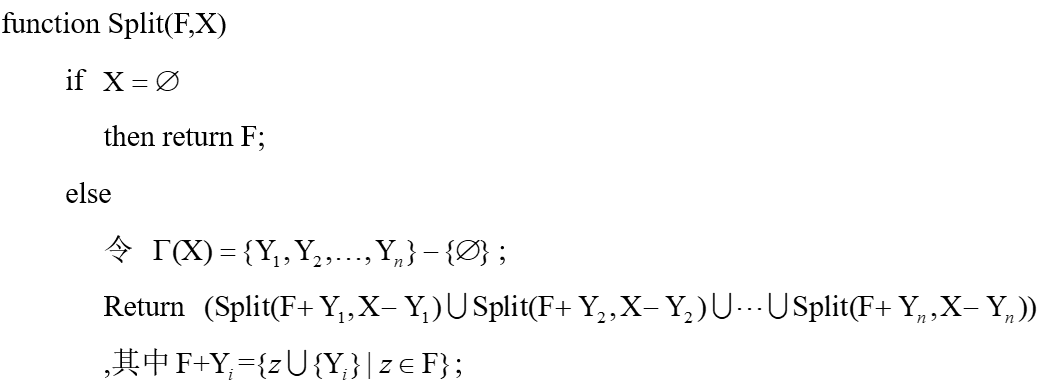
\includegraphics[scale=0.28]{figures/split}
		\end{figure}
	\end{frame}
	
	\begin{frame}{手牌拆分算法模块}
		\text{{\textbf{基于“斗地主”规则的手牌较小拆分算法(LessSplit)}}}
		\begin{figure}
			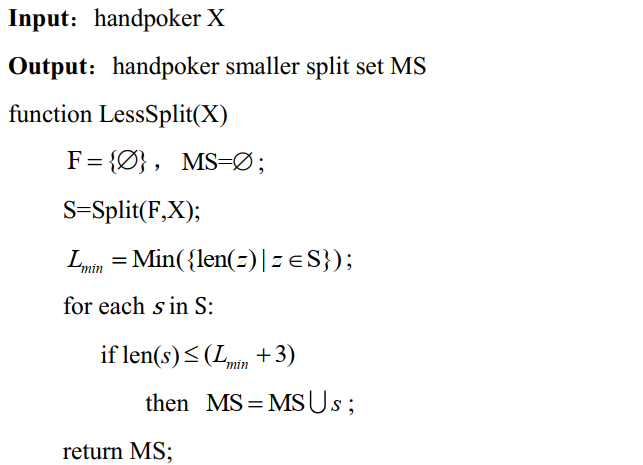
\includegraphics[scale=0.4]{figures/jiyushoupai}
		\end{figure}
	\end{frame}
	
	\begin{frame}
		\frametitle{~~手牌拆分算法实例}
		\begin{itemize}
			\item 玩家的手牌为: 34556789LB。对玩家手牌进行拆分,所有拆分结果为:
			\begin{itemize}
				\item<2-> $s_1$=\{3,4, 5, 5, 6,7, 8, 9, L, B\}
				\item<2-> $s_2$=\{3, 4, 5, 5, 6, 7, 8, 9, LB\}
				\item<2-> $s_3$=\{3, 4, 55, 6, 7, 8, 9, L, B\}
				\item<2-> $s_4$=\{3, 4, 55, 6, 7, 8, 9, LB\}
				\item<2-> $s_5$=\{3, 4, 5, LB, 56789\}
				\item<2-> $s_6$=\{3, 4, 5, L, B, 56789\}
				\item<2-> $s_7$=\{3, 5, 9, LB, 45678\}
				\item<2-> $s_8$=\{3, 5, 9, L, B, 45678\}
				\item<2-> $s_9$=\{3, 5, LB, 456789\}
				\item<2-> $s_{10}$=\{3, 5, L, B, 456789\}
				\item<2-> $s_{11}$=\{5, 8, 9, LB, 34567\}
				\item<2-> $s_{12}$=\{5, 8, 9, L, B, 34567\}
				\item<2-> $s_{13}$=\{5, 9, LB, 345678\}
				\item<2-> $s_{14}$=\{5, 9, L, B, 345678\}
				\item<2-> $s_{15}$=\{5, LB, 3456789\}
				\item<2-> $s_{16}$=\{5, L, B, 3456789\}
			\end{itemize}
		\end{itemize}
	\end{frame}
	
	
	\begin{frame}
		\frametitle{~~手牌拆分算法实例}
		\begin{itemize}
			\item 玩家的手牌为: 34556789LB。对玩家手牌进行拆分,所有拆分结果为:
			\begin{itemize}
				\item<1-> $s_1$=\{3,4, 5, 5, 6,7, 8, 9, L, B\}
				\item<1-> $s_2$=\{3, 4, 5, 5, 6, 7, 8, 9, LB\}
				\item<1-> $s_3$=\{3, 4, 55, 6, 7, 8, 9, L, B\}
				\item<1-> $s_4$=\{3, 4, 55, 6, 7, 8, 9, LB\}
				\item<1-> $s_5$=\{3, 4, 5, LB, 56789\}
				\item<1-> $s_6$=\{3, 4, 5, L, B, 56789\}
				\item<1-> $s_7$=\{3, 5, 9, LB, 45678\}
				\item<1-> $s_8$=\{3, 5, 9, L, B, 45678\}
				\item<1-> $s_9$=\{3, 5, LB, 456789\}
				\item<1-> $s_{10}$=\{3, 5, L, B, 456789\}
				\item<1-> $s_{11}$=\{5, 8, 9, LB, 34567\}
				\item<1-> $s_{12}$=\{5, 8, 9, L, B, 34567\}
				\item<1-> $s_{13}$=\{5, 9, LB, 345678\}
				\item<1-> $s_{14}$=\{5, 9, L, B, 345678\}
				\item<1-> \uuline{$s_{15}$=\{5, LB, 3456789\}}
				\item<1-> $s_{16}$=\{5, L, B, 3456789\}
			\end{itemize}
		\end{itemize}
	\end{frame}
	
	\begin{frame}
		\frametitle{~~手牌拆分算法实例}
		\begin{itemize}
			\item 玩家的手牌为: 34556789LB。对玩家手牌进行拆分,所有拆分结果为:
			\begin{itemize}
				\item<1-> \uwave{$s_1$=\{3,4, 5, 5, 6,7, 8, 9, L, B\}}
				\item<1-> \uwave{$s_2$=\{3, 4, 5, 5, 6, 7, 8, 9, LB\}}
				\item<1-> \uwave{$s_3$=\{3, 4, 55, 6, 7, 8, 9, L, B\}}
				\item<1-> \uwave{$s_4$=\{3, 4, 55, 6, 7, 8, 9, LB\}}
				\item<1-> $s_5$=\{3, 4, 5, LB, 56789\}
				\item<1-> $s_6$=\{3, 4, 5, L, B, 56789\}
				\item<1-> $s_7$=\{3, 5, 9, LB, 45678\}
				\item<1-> $s_8$=\{3, 5, 9, L, B, 45678\}
				\item<1-> $s_9$=\{3, 5, LB, 456789\}
				\item<1-> $s_{10}$=\{3, 5, L, B, 456789\}
				\item<1-> $s_{11}$=\{5, 8, 9, LB, 34567\}
				\item<1-> $s_{12}$=\{5, 8, 9, L, B, 34567\}
				\item<1-> $s_{13}$=\{5, 9, LB, 345678\}
				\item<1-> $s_{14}$=\{5, 9, L, B, 345678\}
				\item<1-> \uuline{$s_{15}$=\{5, LB, 3456789\}}
				\item<1-> $s_{16}$=\{5, L, B, 3456789\}
			\end{itemize}
		\end{itemize}
	\end{frame}
	
	\begin{frame}
		\frametitle{~~手牌拆分算法实例}
		\begin{itemize}
			\item 玩家的手牌为: 34556789LB。对玩家手牌进行拆分,所有拆分结果为:
			\begin{itemize}
				\item<1-> \uwave{$s_1$=\{3,4, 5, 5, \textcolor{red}{\textbf{6}},\textcolor{red}{\textbf{7}}, 8, 9, L, B\}}
				\item<1-> \uwave{$s_2$=\{3, 4, 5, 5, \textcolor{red}{\textbf{6}}, \textcolor{red}{\textbf{7}}, 8, 9, LB\}}
				\item<1-> \uwave{$s_3$=\{3, 4, \textcolor{red}{\textbf{55}}, \textcolor{red}{\textbf{6}}, \textcolor{red}{\textbf{7}}, 8, 9, L, B\}}
				\item<1-> \uwave{$s_4$=\{3, 4, \textcolor{red}{\textbf{55}}, \textcolor{red}{\textbf{6}}, \textcolor{red}{\textbf{7}}, 8, 9, LB\}}
				\item<1-> $s_5$=\{3, 4, 5, LB, 56789\}
				\item<1-> $s_6$=\{3, 4, 5, L, B, 56789\}
				\item<1-> $s_7$=\{3, 5, 9, LB, 45678\}
				\item<1-> $s_8$=\{3, 5, 9, L, B, 45678\}
				\item<1-> $s_9$=\{3, 5, LB, 456789\}
				\item<1-> $s_{10}$=\{3, 5, L, B, 456789\}
				\item<1-> $s_{11}$=\{5, 8, 9, LB, 34567\}
				\item<1-> $s_{12}$=\{5, 8, 9, L, B, 34567\}
				\item<1-> $s_{13}$=\{5, 9, LB, 345678\}
				\item<1-> $s_{14}$=\{5, 9, L, B, 345678\}
				\item<1-> \uuline{$s_{15}$=\{5, LB, 3456789\}}
				\item<1-> $s_{16}$=\{5, L, B, 3456789\}
			\end{itemize}
		\end{itemize}
	\end{frame}
	
	\subsection*{蒙特卡洛树搜索算法}
	\begin{frame}
		\frametitle{~~蒙特卡洛树搜索算法}
		\begin{block}{蒙特卡洛抽样法}
			~~~为了求解问题,首先建立一个概率模型或随机过程,使它的参数或数字特征等于问题的解,然后通过对模型、过程的观察或者抽样试验来计算这些参数、数字特征,最后给出所求解的近似值。 \\
		\end{block}
		\text{如:Buffon's needle problem}
		\begin{figure}
			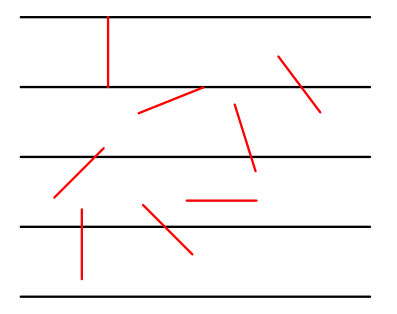
\includegraphics[scale=0.5]{figures/Buffon}
		\end{figure}
	\end{frame}
	
	
	\begin{frame}
		\frametitle{~~蒙特卡洛树搜索算法}
		\text{博弈树搜索算法:将初始状态和所有可能的后续状态通过直接先}
		\text{后关系连接在一起形成博弈树}
		\begin{figure}
			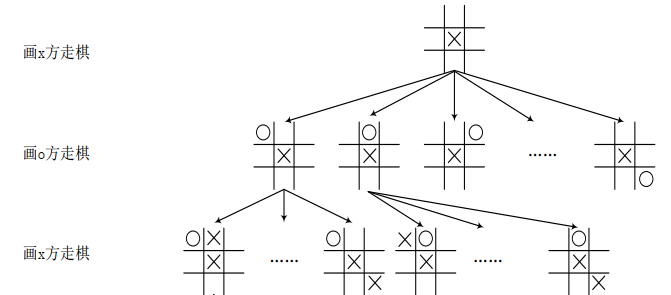
\includegraphics[scale=0.5]{figures/bytree}
		\end{figure}
	\end{frame}
	
	
	\begin{frame}
		\frametitle{~~蒙特卡洛树搜索算法}
		\begin{columns}
			\column<1->{0.5\textwidth}
			\begin{figure}
				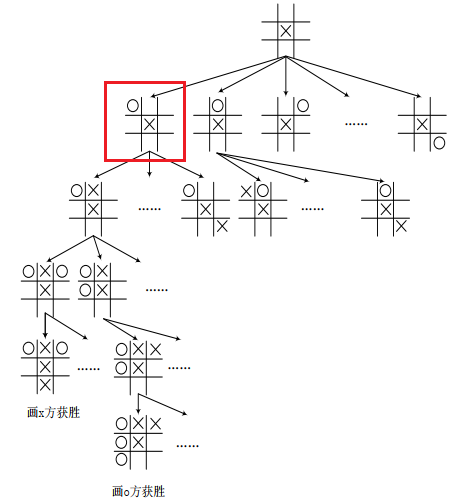
\includegraphics[scale=0.5]{figures/jtree}
			\end{figure}
			
			\column{0.5\textwidth}
			\begin{block}{思想}
				~~~利用经验平均来代替随机变量的期望。如在博弈状态$s$时期望值为$v_{\pi}(s)$,一般难以通过计
				算直接求出该值,但是可以通过蒙特卡洛方法获得一系列收益$G_1(s)$,$\cdots$,$G_n(s)$.根据大数定律,当$n$趋于无穷大时,抽样收益的均值趋近于期望值。定义$v(s)$ 为系列收益的平均值,即
				$$v(s)=\frac{G_1(s)+\cdots+G_n(s)}{n}$$
				\begin{center} 当$n \to \infty$时,$v(s) \rightarrow v_{\pi}(s)$ \end{center}
			\end{block}
		\end{columns}
	\end{frame}
	
	\begin{frame}
		\frametitle{~~蒙特卡洛树搜索算法}
		\Large \text{蒙特卡洛树搜索算法过程} 
		\begin{figure}
			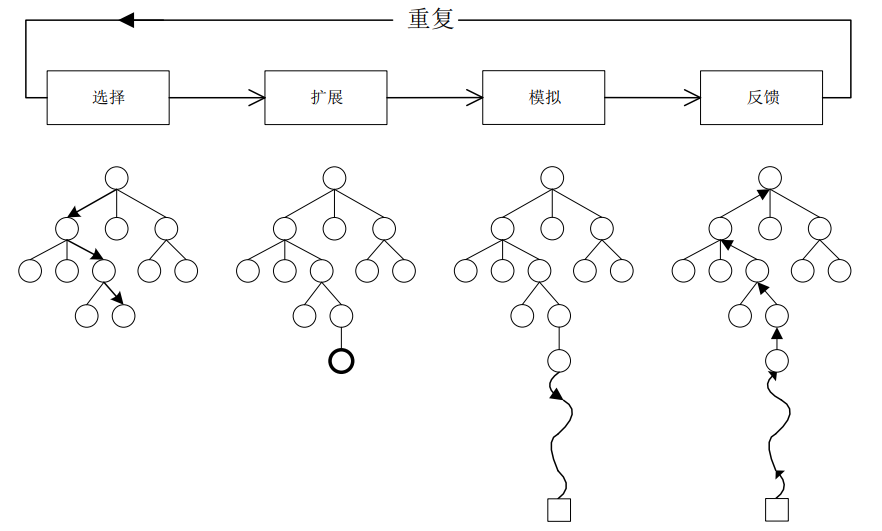
\includegraphics[scale=0.5]{figures/MCTS}
		\end{figure}
	\end{frame}
	
	\subsection*{基于手牌拆分的蒙特卡洛树搜索算法}
	\begin{frame}{~~基于手牌拆分的蒙特卡洛树搜索算法}{~~~~(MCTSHS)}
		\Large \text{基于手牌拆分的蒙特卡洛树搜索算法过程} 
		\begin{figure}
			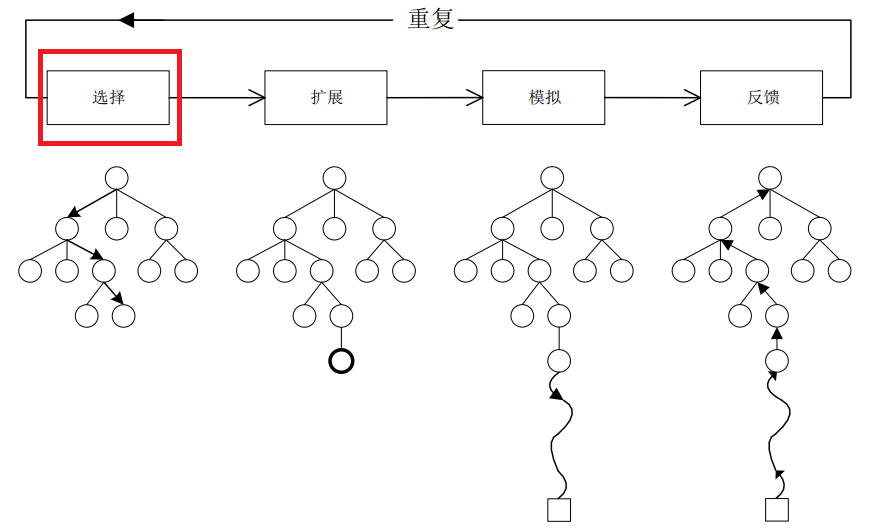
\includegraphics[scale=0.5]{figures/MCTSCF}
		\end{figure}
	\end{frame}
	
	\subsection*{实验比较结果}
	\begin{frame}
		\frametitle{~~与规则算法(RB)比较}
		\begin{block}{规则算法(RB)}
			~~~~该算法分为主动策略和被动策略两种。主动策略中若上轮玩家取得主动权,那本轮该玩家可根据自己手牌主动选择出牌类型,而不需要考虑其他玩家的出牌类型;被动策略中玩家需要考虑本轮其他玩家的出牌, 被动选择跟牌类型。 
		\end{block}
		\text{不区分角色比较结果:}
		\begin{figure}
			\includegraphics<2->[scale=0.4]{figures/AllMvR}
		\end{figure}
	\end{frame}
	
	\begin{frame}
		\frametitle{~~与规则算法(RB)比较}
		\text{地主MCTSHS对农民RB:}
		\begin{figure}
			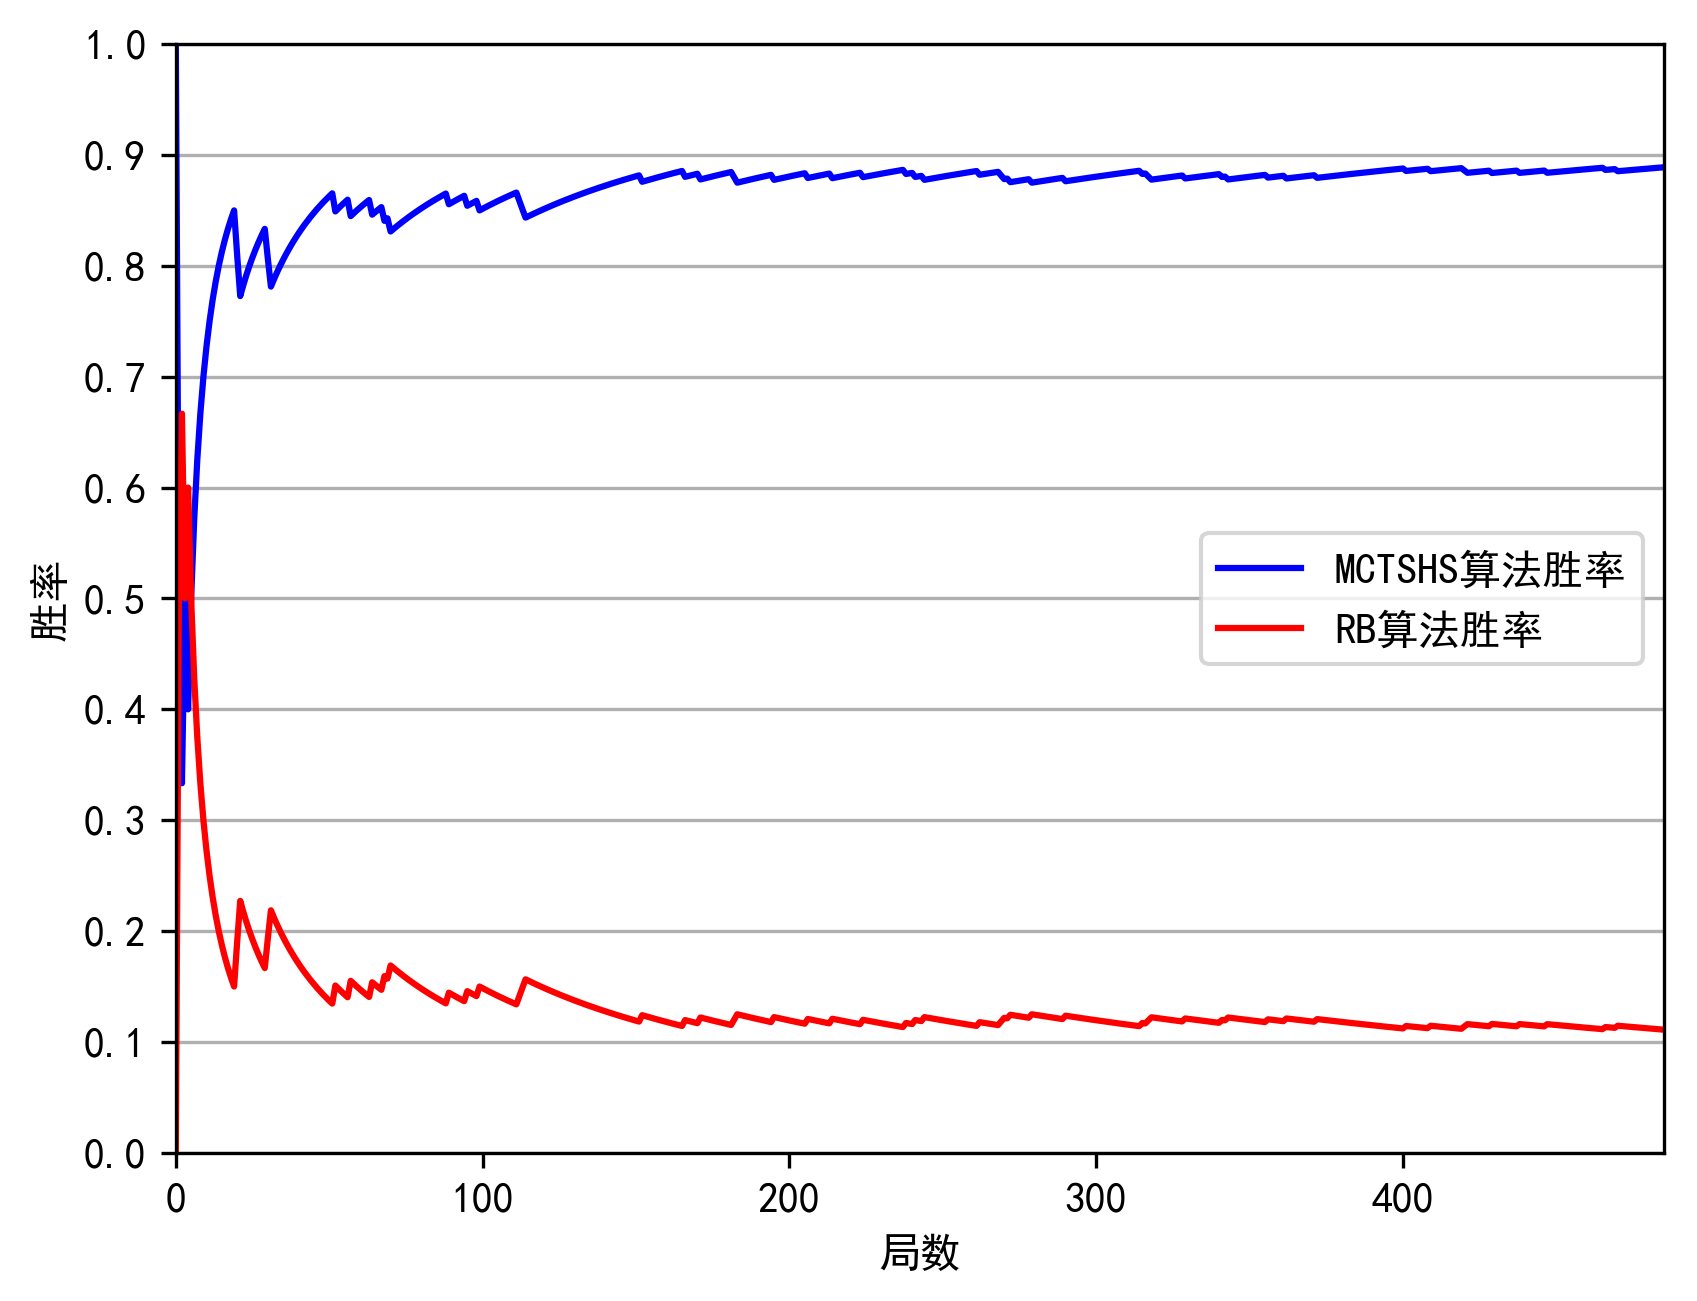
\includegraphics[scale=0.6]{figures/MvR}
		\end{figure}
	\end{frame}
	
	\begin{frame}
		\frametitle{~~与规则算法(RB)比较}
		\text{农民MCTSHS对地主RB:}
		\begin{figure}
			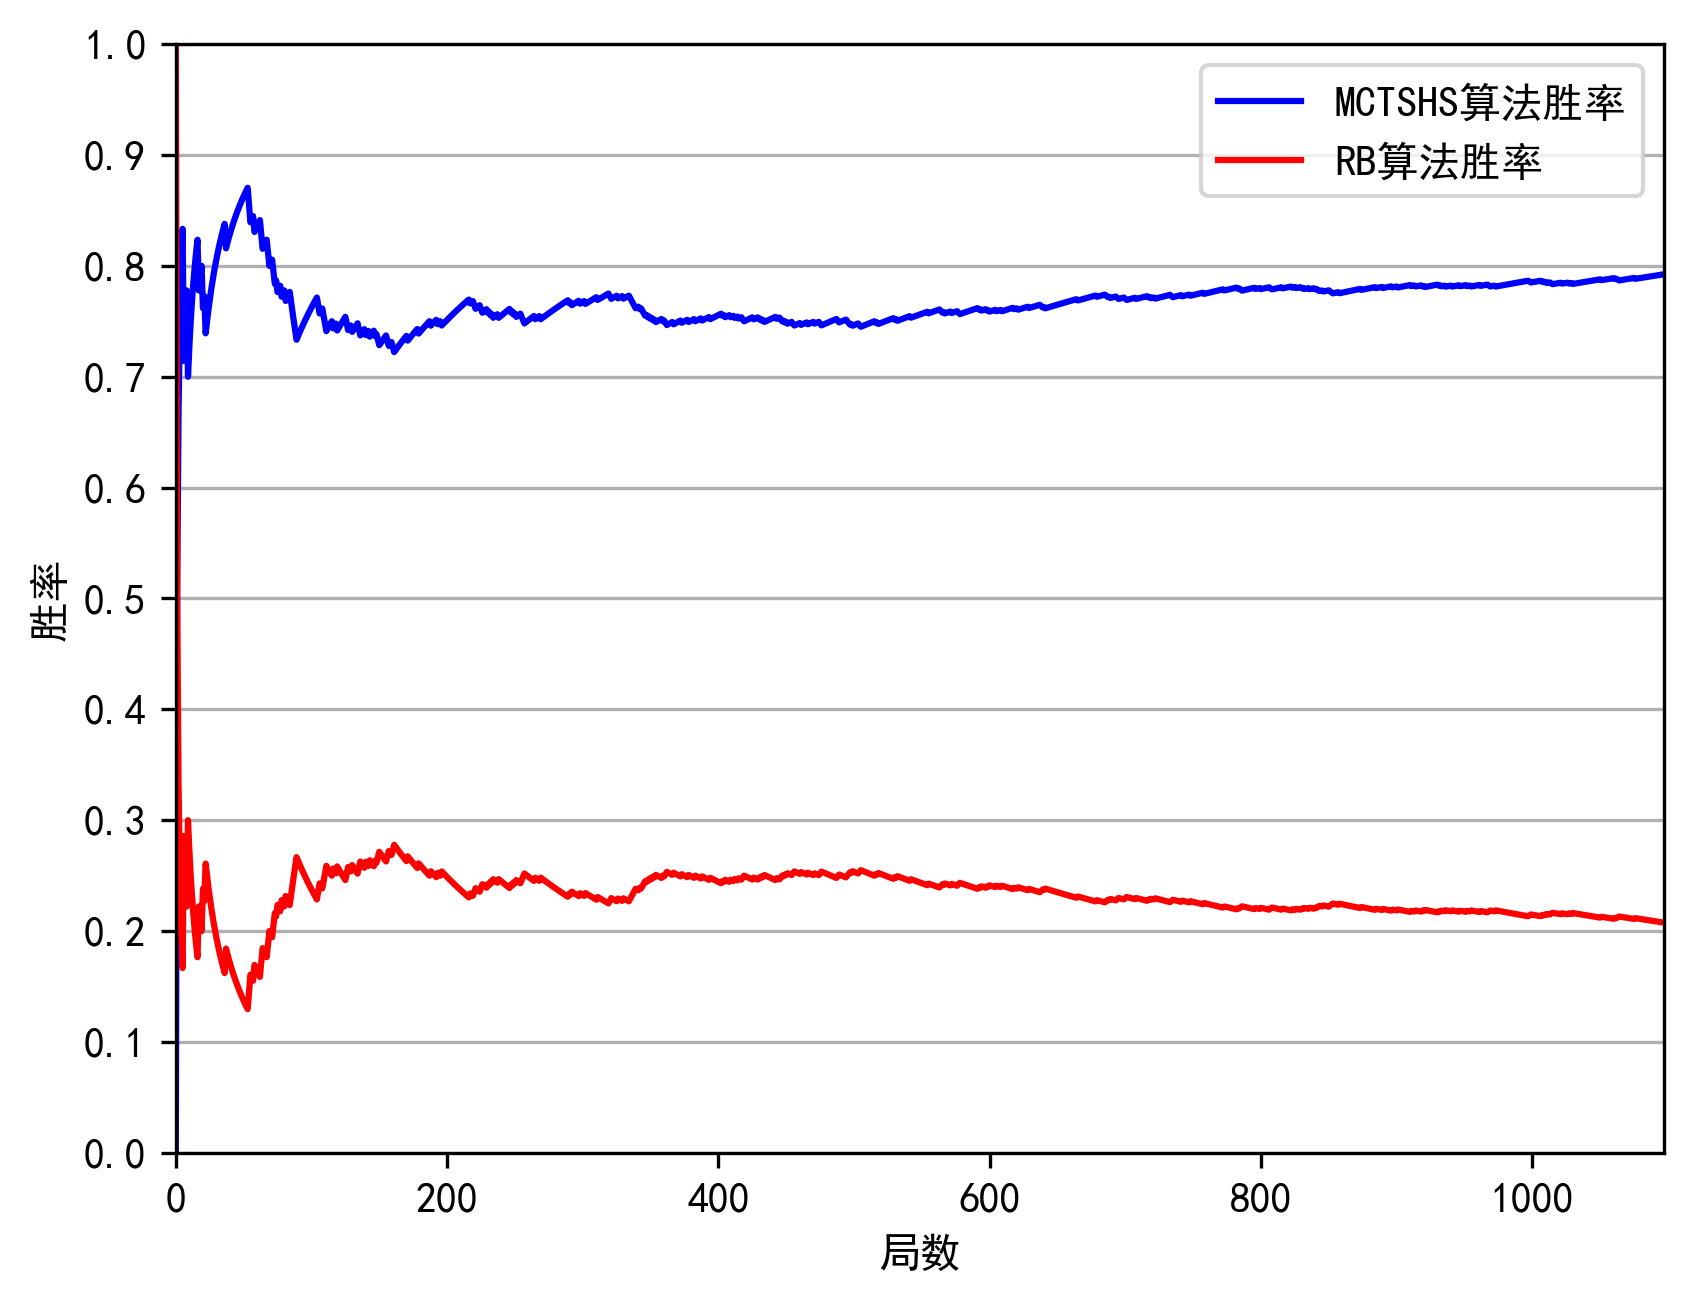
\includegraphics[scale=0.6]{figures/RvM}
		\end{figure}
	\end{frame}
	
	\begin{frame}
		\frametitle{~~与7k7k算法比较}
		\begin{block}{7k7k算法}
			~~~~该算法为北京迦游网络科技有限公司开发的“斗地主”智能算法。 
		\end{block}
		\text{不区分角色比较结果:}
		\begin{figure}
			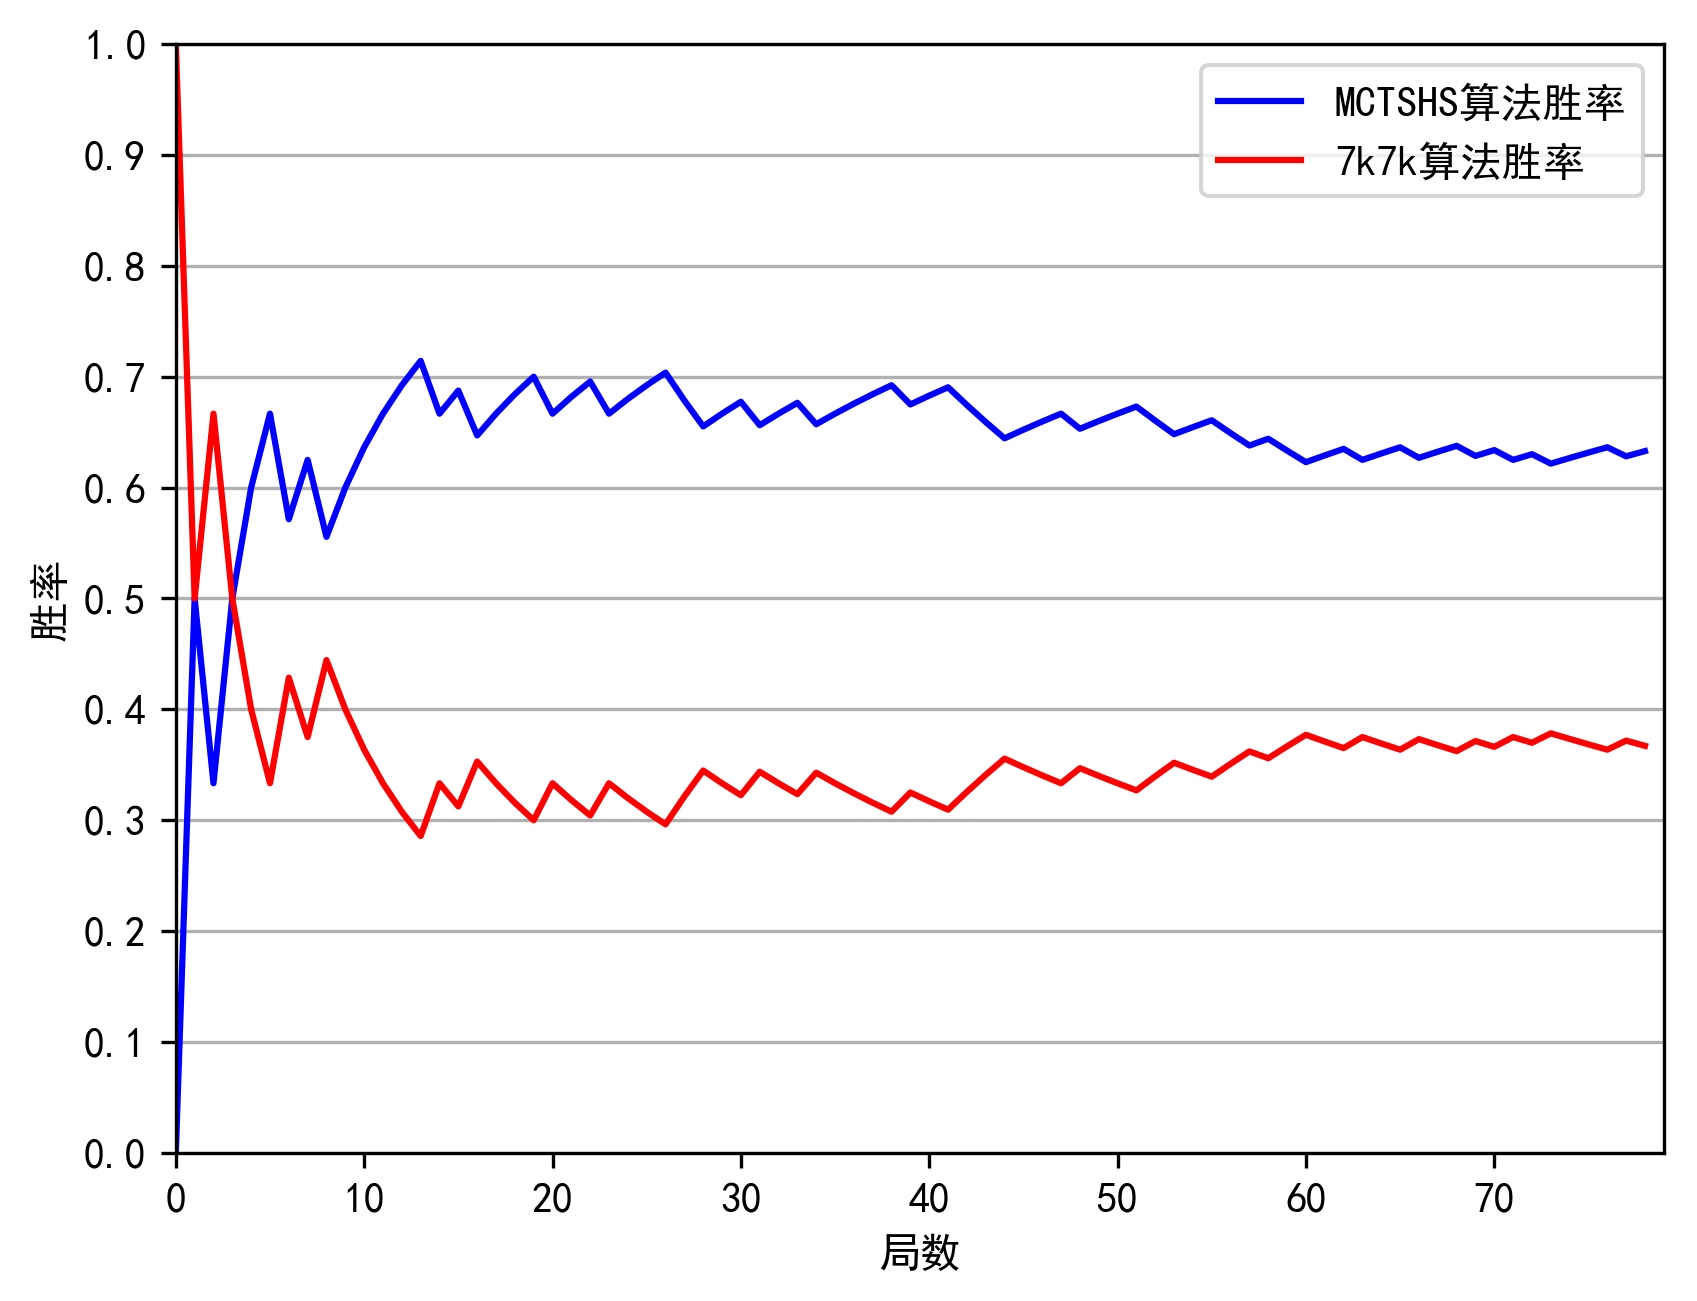
\includegraphics[scale=0.5]{figures/Mv7k7k}
		\end{figure}
	\end{frame}
	
	\subsection*{合作问题分析}
	\begin{frame}
		\frametitle{~~合作问题分析}
		\text{合作问题分析:}
		\begin{figure}
			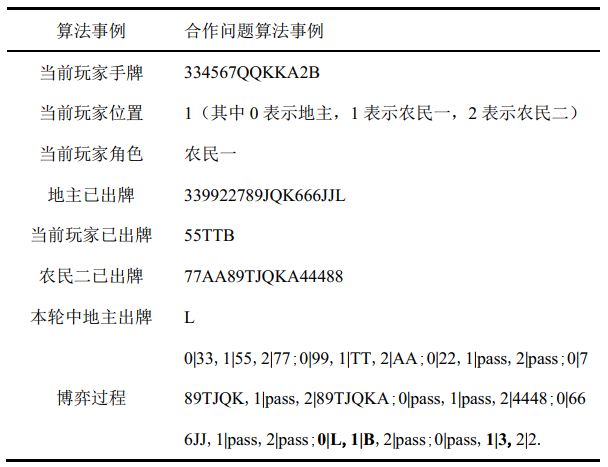
\includegraphics[scale=0.7]{figures/hz}
		\end{figure}
	\end{frame}
	
	\subsection*{算法缺点}
	\begin{frame}
		\frametitle{~~算法缺点}
		\begin{spacing}{2.0}
			\text{算法缺点:}
			\begin{itemize}
				\item 每次决策思考时间过长
				\item 已搜索到的决策未能充分利用
			\end{itemize}
		\end{spacing}
	\end{frame}
	
	\begin{frame}
		\frametitle{~~算法缺点}
		\begin{spacing}{2.0}
			\text{算法缺点:}
			\begin{itemize}
				\item<1-> 每次决策思考时间过长
				\item<1-> 已搜索到的决策未能充分利用
			\end{itemize}
		\end{spacing}
		\LARGE \text{{\LARGE 改进算法!!}}
	\end{frame}
	
	\section{结合卷积神经网络的蒙特卡洛树搜索}
	\subsection*{结合卷积神经网络的蒙特卡洛树搜索}
	\begin{frame}
		\frametitle{~结合卷积神经网络的蒙特卡洛树搜索模型MCM}
		\[
		\text{{\Large \textbf{MCM模型}}}
		\begin{cases}
			\text{手牌拆分的蒙特卡洛树搜索模块} \\ \\
			\text{CNN策略学习模块}\\ \\
			\text{改善策略模块}
		\end{cases}
		\]
		\large \text{CNN策略学习模块:} 
		\begin{figure}
			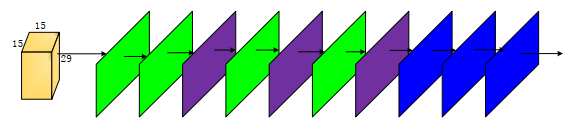
\includegraphics[scale=0.85]{figures/cnn}
		\end{figure}
	\end{frame}
	
	\begin{frame}
		\frametitle{~结合卷积神经网络的蒙特卡洛树搜索模型MCM}
		\[
		\text{{\Large \textbf{MCM模型}}}
		\begin{cases}
			\text{手牌拆分的蒙特卡洛树搜索模块} \\ \\
			\text{CNN策略学习模块}\\ \\
			\text{改善策略模块}
		\end{cases}
		\]
		\large \text{CNN策略学习模块:} 
		\begin{figure}
			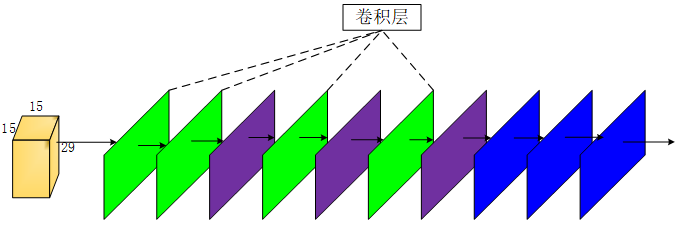
\includegraphics[scale=0.65]{figures/cnn1}
		\end{figure}
	\end{frame}
	
	\begin{frame}
		\frametitle{~结合卷积神经网络的蒙特卡洛树搜索模型MCM}
		\[
		\text{{\Large \textbf{MCM模型}}}
		\begin{cases}
			\text{手牌拆分的蒙特卡洛树搜索模块} \\ \\
			\text{CNN策略学习模块}\\ \\
			\text{改善策略模块}
		\end{cases}
		\]
		\large \text{CNN策略学习模块:} 
		\begin{figure}
			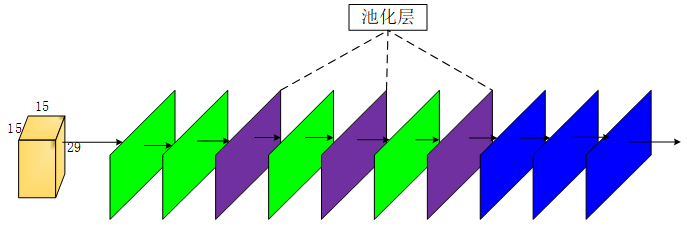
\includegraphics[scale=0.65]{figures/cnn2}
		\end{figure}
	\end{frame}
	
	\begin{frame}
		\frametitle{~结合卷积神经网络的蒙特卡洛树搜索模型MCM}
		\[
		\text{{\Large \textbf{MCM模型}}}
		\begin{cases}
			\text{手牌拆分的蒙特卡洛树搜索模块} \\ \\
			\text{CNN策略学习模块}\\ \\
			\text{改善策略模块}
		\end{cases}
		\]
		\large \text{CNN策略学习模块:} 
		\begin{figure}
			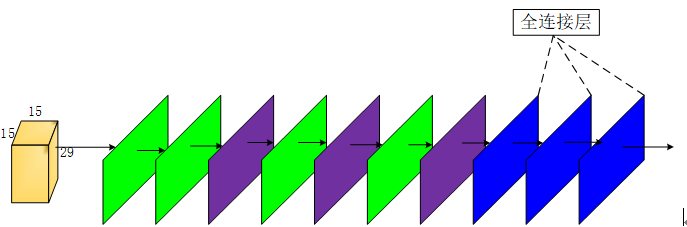
\includegraphics[scale=0.65]{figures/cnn3}
		\end{figure}
	\end{frame}
	
	\begin{frame}
		\frametitle{~结合卷积神经网络的蒙特卡洛树搜索模型MCM}
		\[
		\text{{\Large \textbf{MCM模型}}}
		\begin{cases}
			\text{手牌拆分的蒙特卡洛树搜索模块} \\ \\
			\text{CNN策略学习模块}\\ \\
			\text{改善策略模块}
		\end{cases}
		\]
		\large \text{CNN策略学习模块:} 
		\begin{figure}
			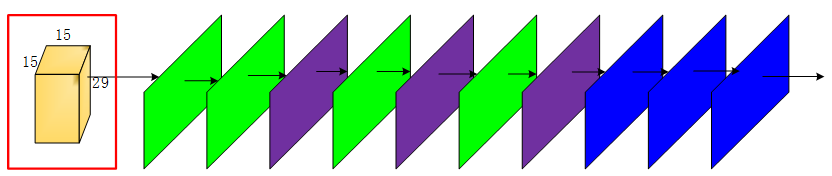
\includegraphics[scale=0.55]{figures/cnnInput}
		\end{figure}
	\end{frame}
	
	\subsection*{CNN策略学习模块}
	\begin{frame}
		\frametitle{~~CNN策略学习模块-----输入表示}
		\begin{itemize}
			\item<1-> X维度:表示15种扑克
			\item<2-> Y维度:
			\begin{itemize}
				\item<3-> 0-3(下标)表示扑克的张数
				\item<4-> 4-13(下标)表示扑克是否参与组成出牌类型
				\item<5-> 14(下标)表示该出牌是否为地主玩家。
			\end{itemize}
			\item<6-> Z维度:\vspace{-0.05cm}\begin{figure}
				\includegraphics<6->[scale=0.6]{figures/z}
			\end{figure}
		\end{itemize}
	\end{frame}
	
	\begin{frame}
		\frametitle{~~CNN策略学习模块}
		\begin{spacing}{2.0}
			\begin{itemize}
				\item 学习样本处理
				\begin{itemize}
					\item 将MCTSHS决策结果的数据进行去重
					\item 随机打乱去重后的样本顺序,并从打乱的样本中,随机选择 90\%的样本组成训练集, 10\%作为测试集
				\end{itemize}
			\end{itemize}
		\end{spacing}
	\end{frame}
	
	\begin{frame}
		\frametitle{~~CNN策略学习模块}
		\begin{spacing}{1.5}
			\begin{itemize}
				\item<1-> 学习样本处理
				\begin{itemize}
					\item<1-> 将MCTSHS决策结果的数据进行去重
					\item<1-> 随机打乱去重后的样本顺序,并从打乱的样本中,随机选择 90\%的样本组成训练集, 10\%作为测试集
				\end{itemize}
			\end{itemize}
		\end{spacing}
		\text{\textbf{MCTSHS学习的部分历史数据记录:}}
		\begin{figure}
			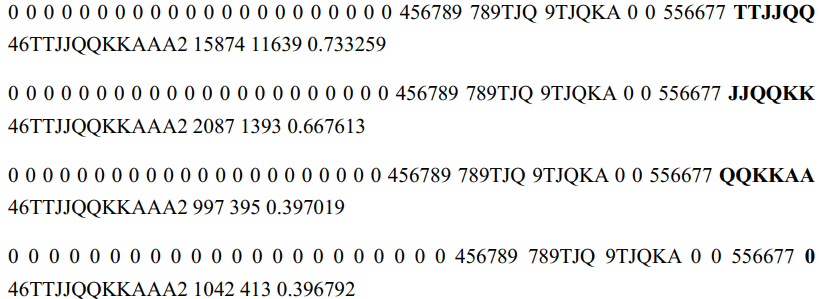
\includegraphics[scale=0.35]{figures/sample}
		\end{figure}
	\end{frame}
	
	\begin{frame}
		\frametitle{~~CNN策略学习模块}
		\text{CNN网络学习策略损失变化图:}
		\begin{figure}
			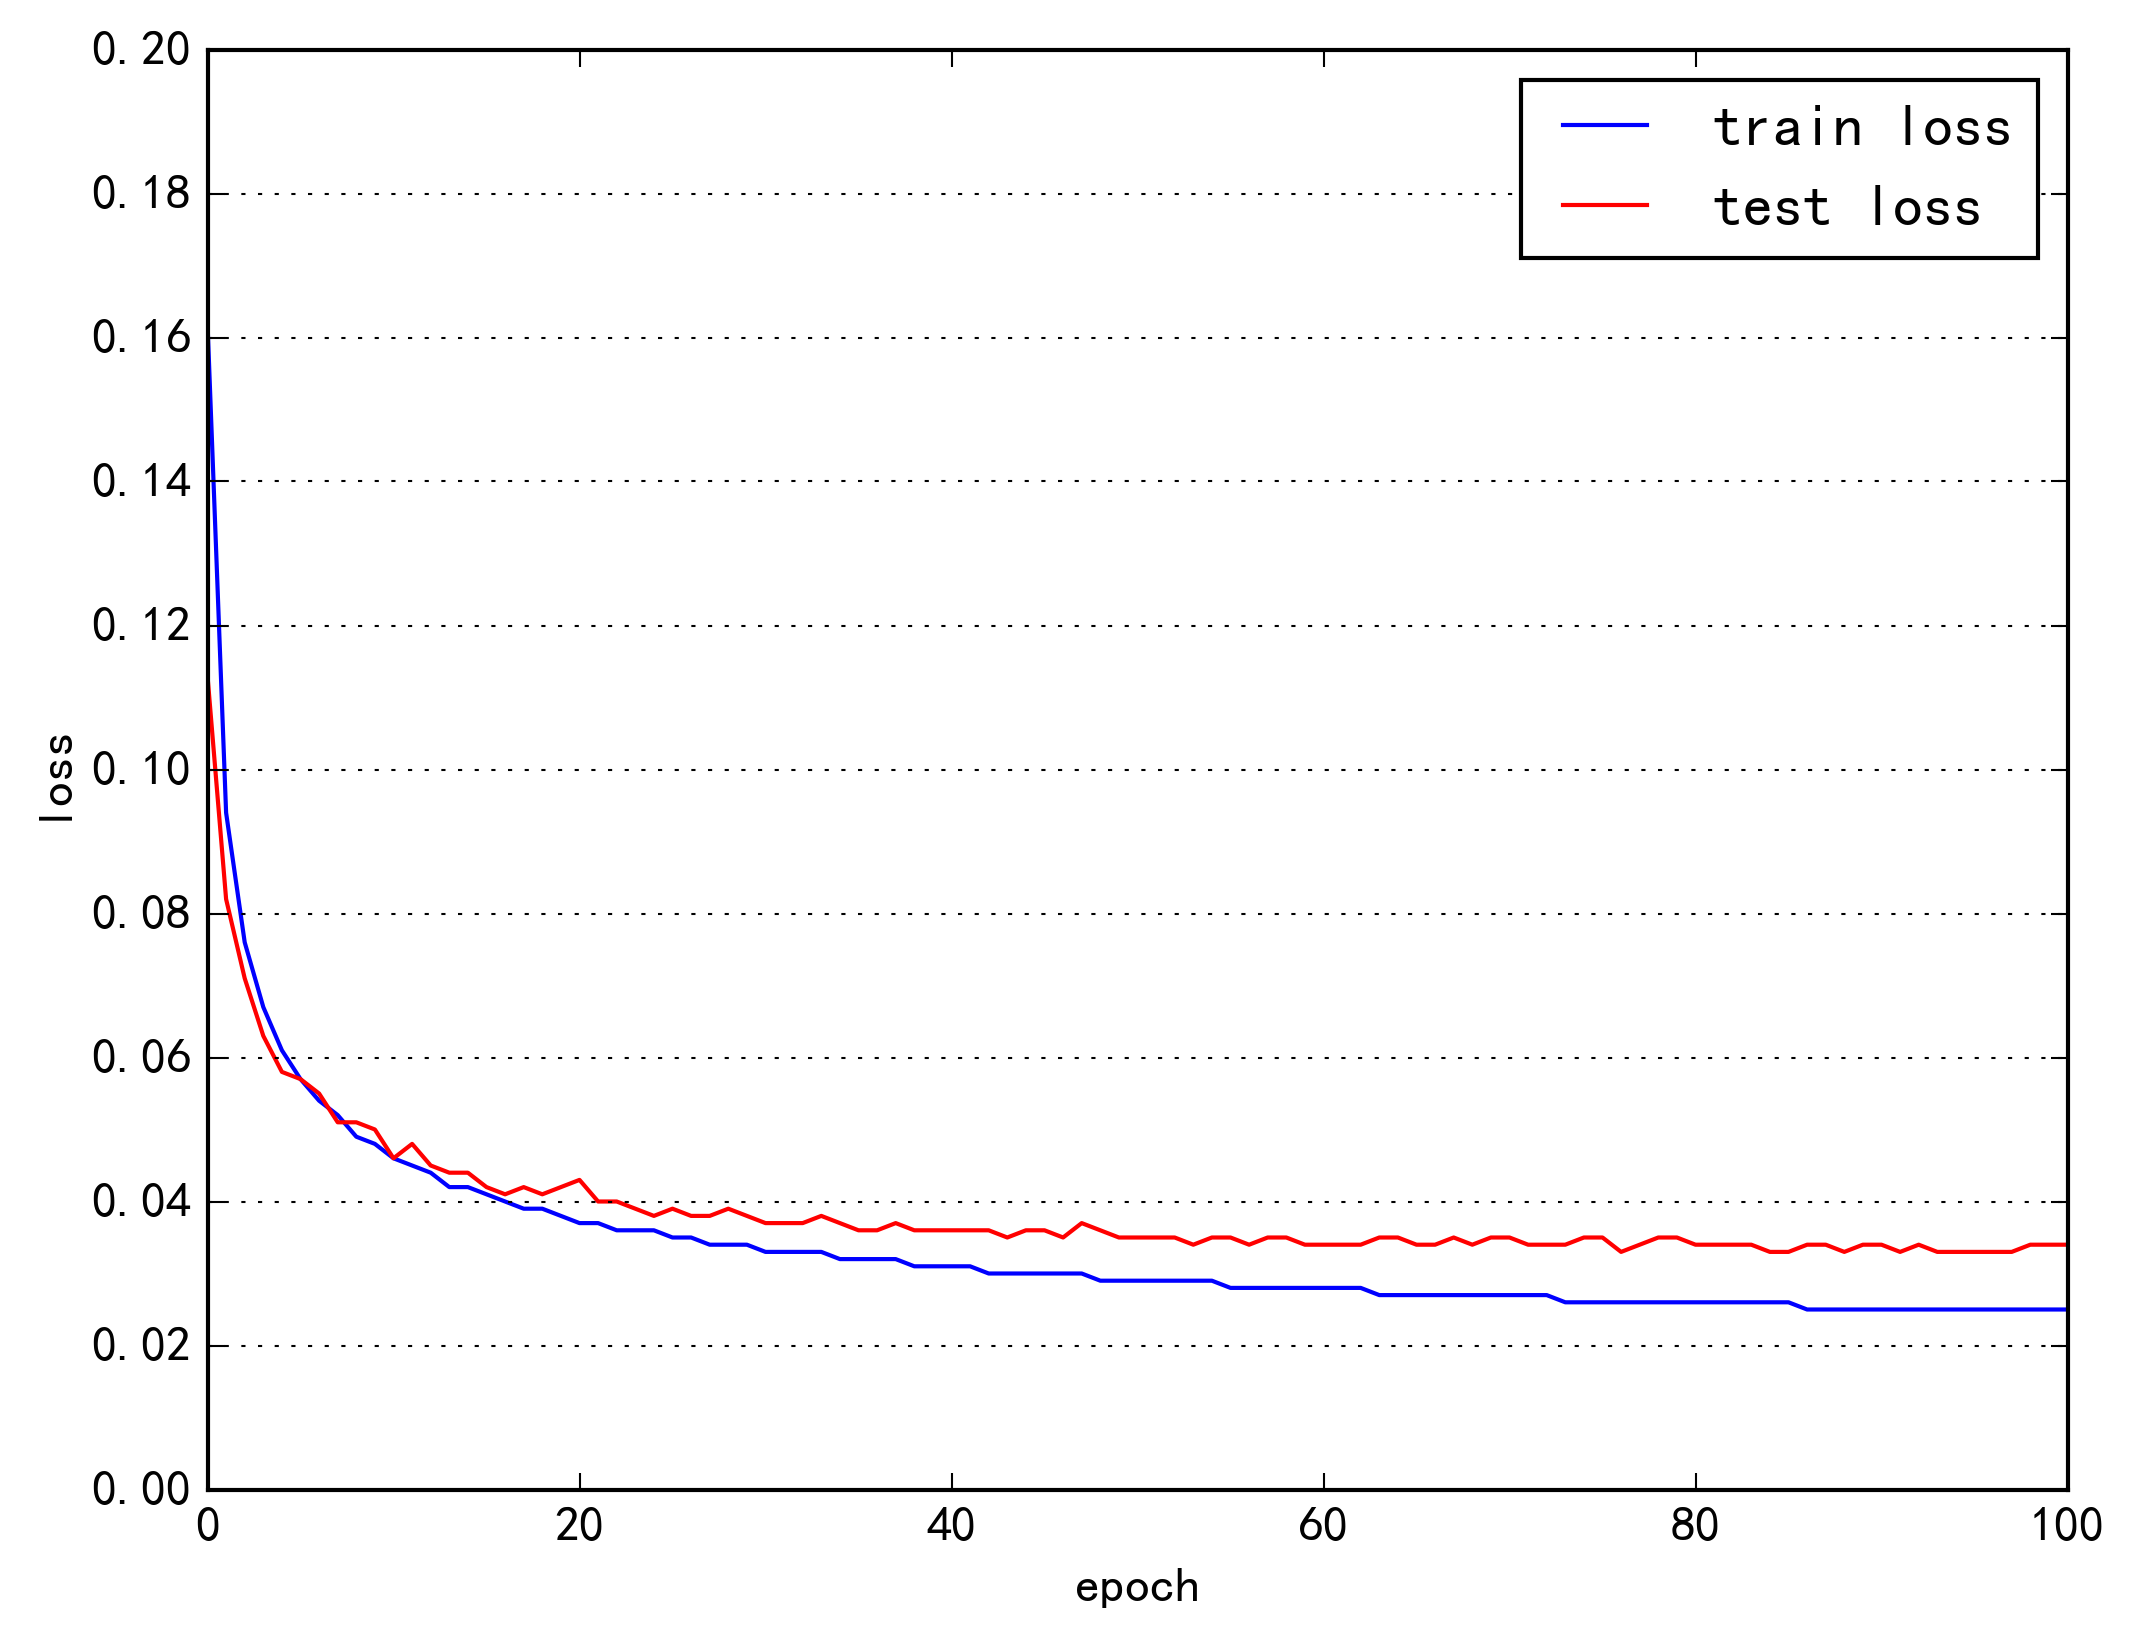
\includegraphics[scale=0.5]{figures/loss}
		\end{figure}
	\end{frame}
	
	\subsection*{实验结果}
	\begin{frame}
		\frametitle{~~实验结果-----实验比较设定}
		\text{实验比较设定}
		\begin{itemize}
			\item 地主、农民使用不同的决策算法,其中农民一、农民二均使用农民的决策算法
			\item 地主、农民一、农民二使用不同的决策算法
			\item 地主、农民一、农民二使用不同的决策算法进行相同牌局比较
		\end{itemize}
	\end{frame}
	
	\begin{frame}
		\frametitle{~~实验结果-----与随机算法(Random)比较}
		\begin{block}{随机算法(Random)介绍}
			~~~~思路为:根据玩家的手牌、 本轮其它玩家出牌等信息按照博弈规则计算出当前状态下玩家可能的所有出牌, 并从中随机选择一种可能出牌作为本轮的最终出牌。
		\end{block}
		\text{地主 MCM 对农民 Random 的胜率变化图:}\vspace{-0.1cm}
		\begin{figure}
			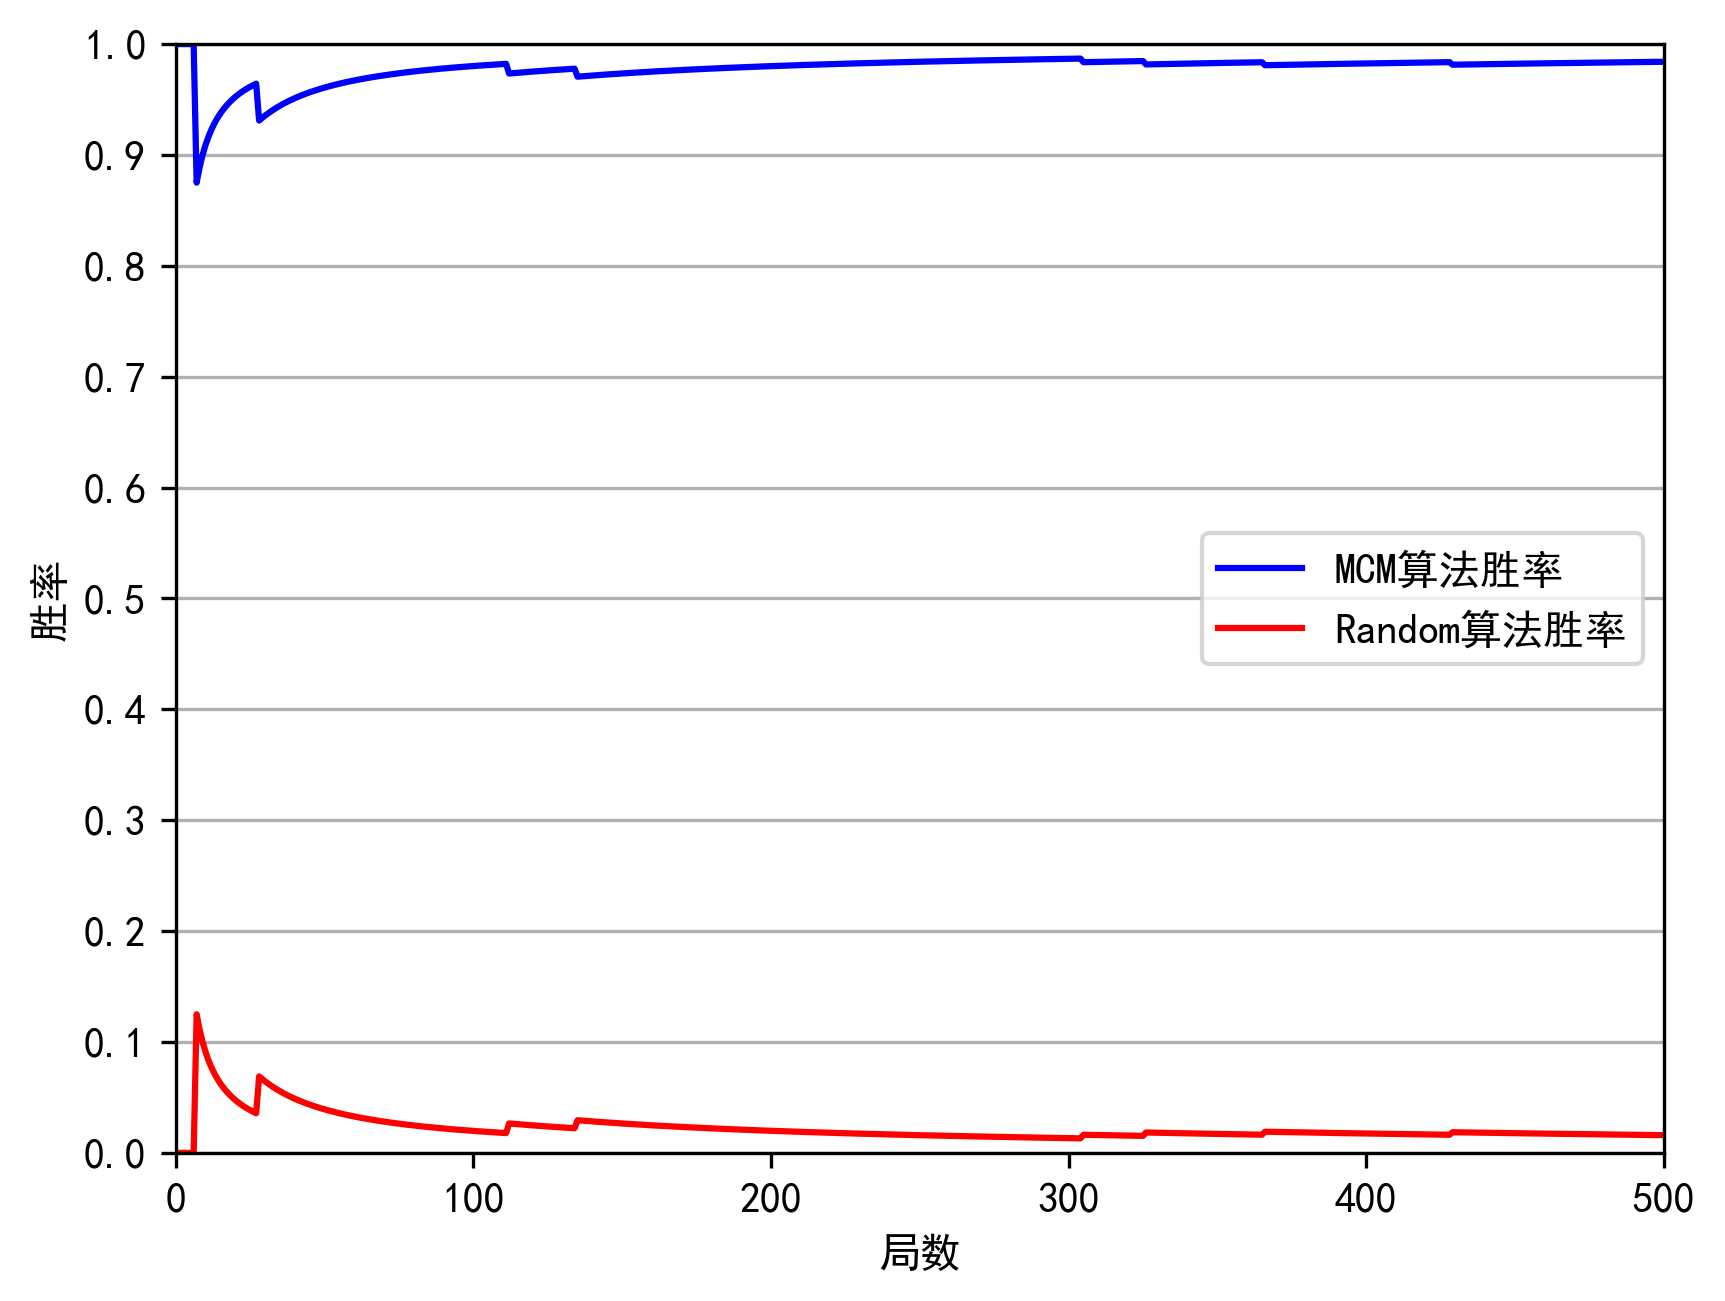
\includegraphics[scale=0.45]{figures/MCvR}
		\end{figure}
	\end{frame}
	
	\begin{frame}
		\frametitle{~~实验结果-----与随机算法(Random)比较}
		\text{农民MCM 对地主Random 的胜率变化图:}\vspace{-0.1cm}
		\begin{figure}
			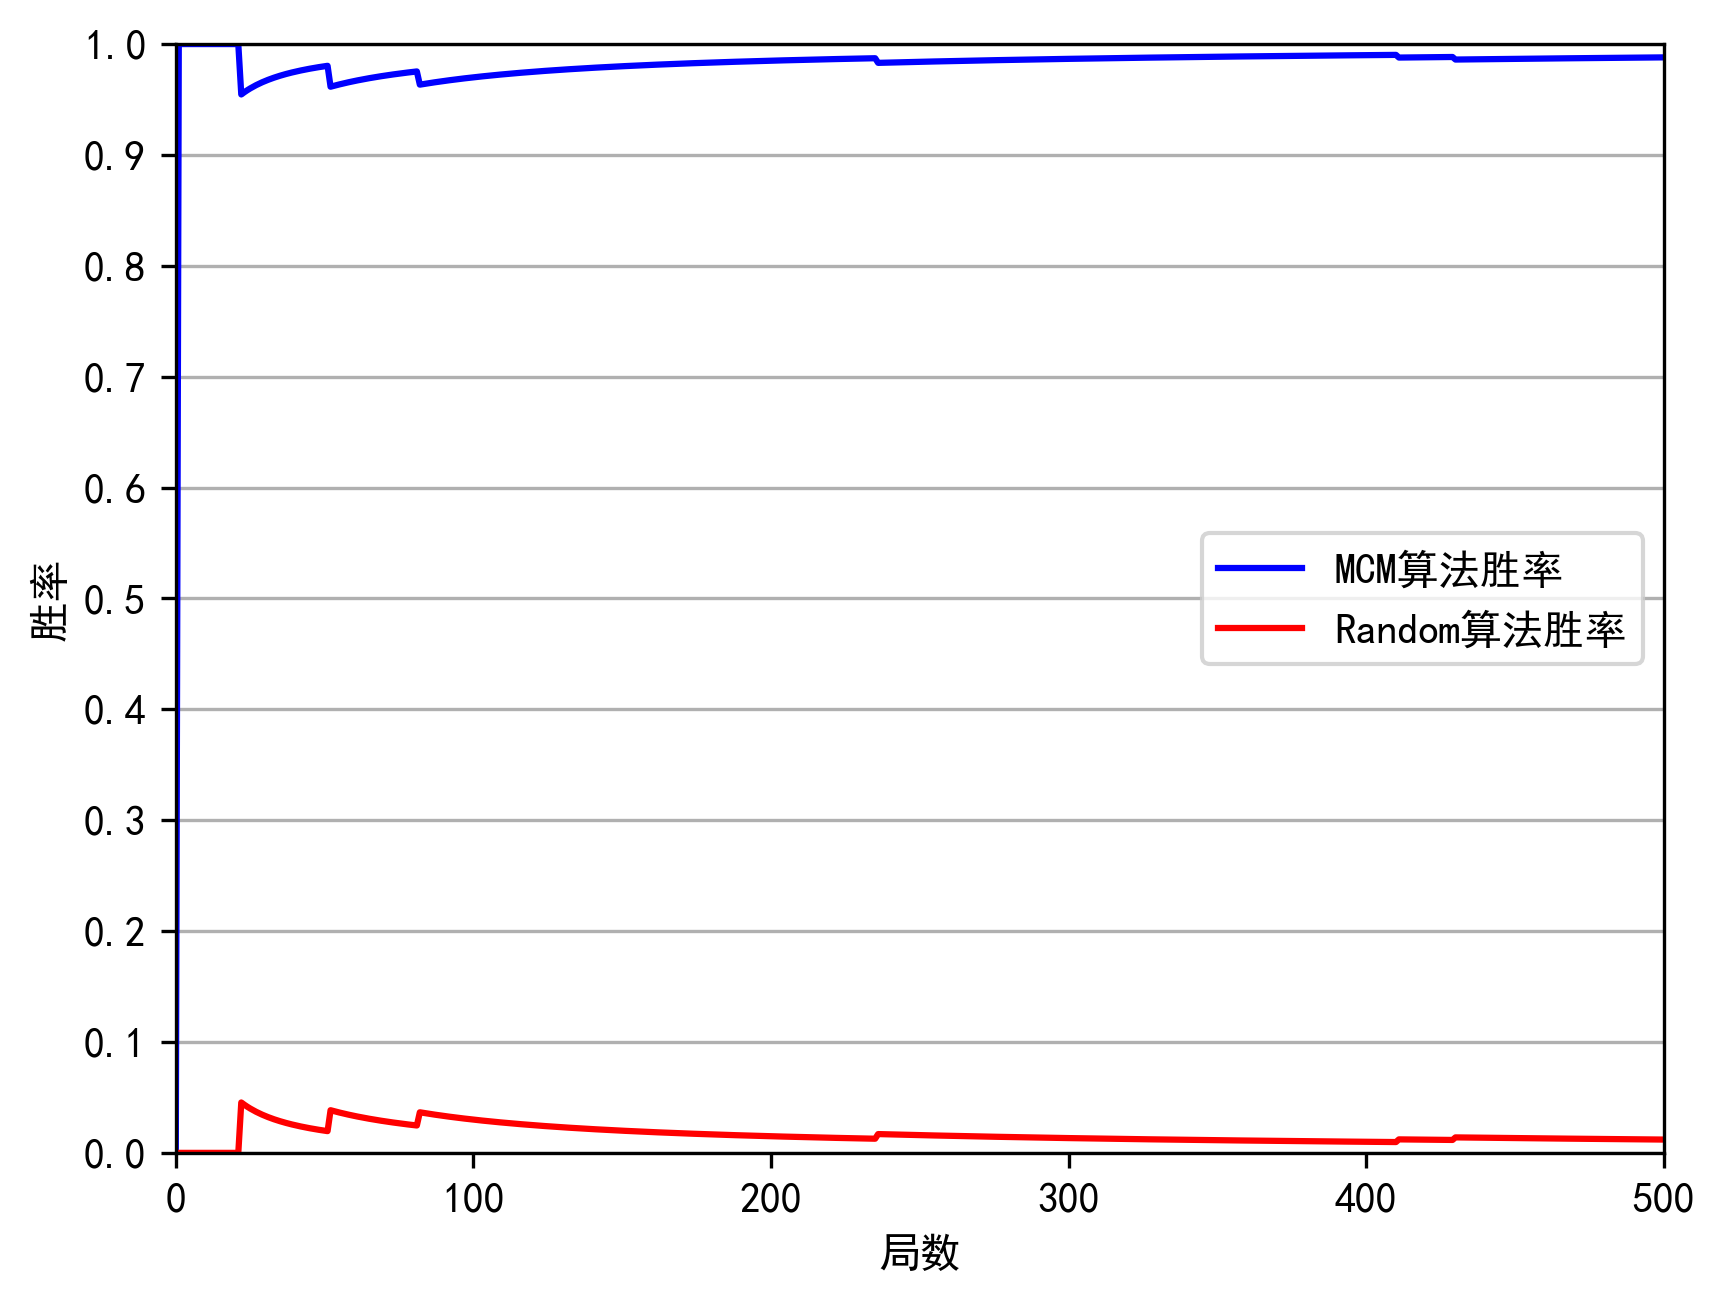
\includegraphics[scale=0.6]{figures/RvMC}
		\end{figure}
	\end{frame}
	
	
	\begin{frame}
		\frametitle{~~实验结果-----与RHCP算法比较}
		\begin{block}{RHCP算法介绍}
			~~~~该算法引入手牌剩余价值的概念,其总体思路是将手牌按照“斗地主”规则进行不同的组合,并选择使得出牌后手牌价值较高的出牌作为本轮最佳出牌。
		\end{block}
		\text{地主 MCM 对农民 RHCP 的胜率变化图:}\vspace{-0.1cm}
		\begin{figure}
			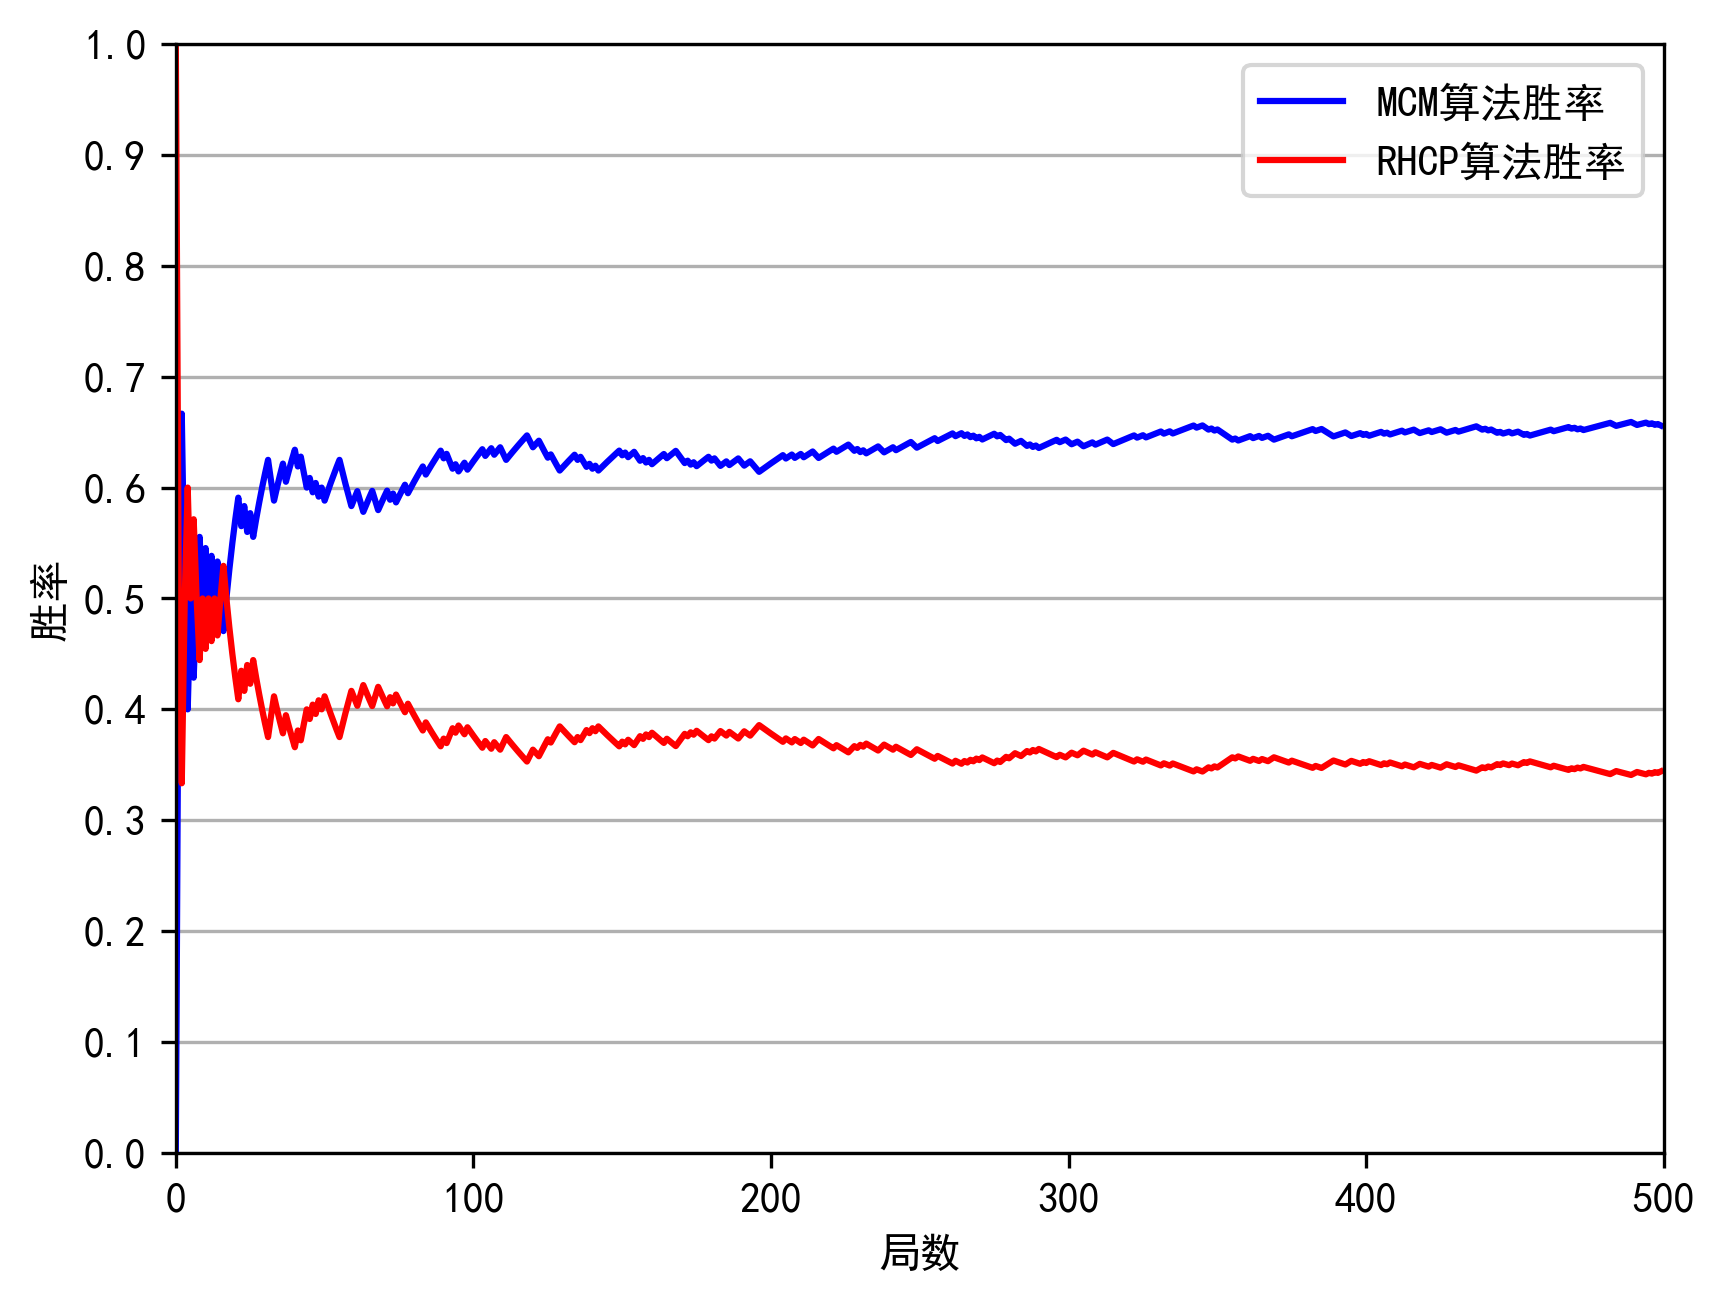
\includegraphics[scale=0.45]{figures/MCvRHCP}
		\end{figure}
	\end{frame}
	
	\begin{frame}
		\frametitle{~~实验结果-----与RHCP算法比较}
		\text{农民MCM 对地主RHCP 的胜率变化图:}\vspace{-0.1cm}
		\begin{figure}
			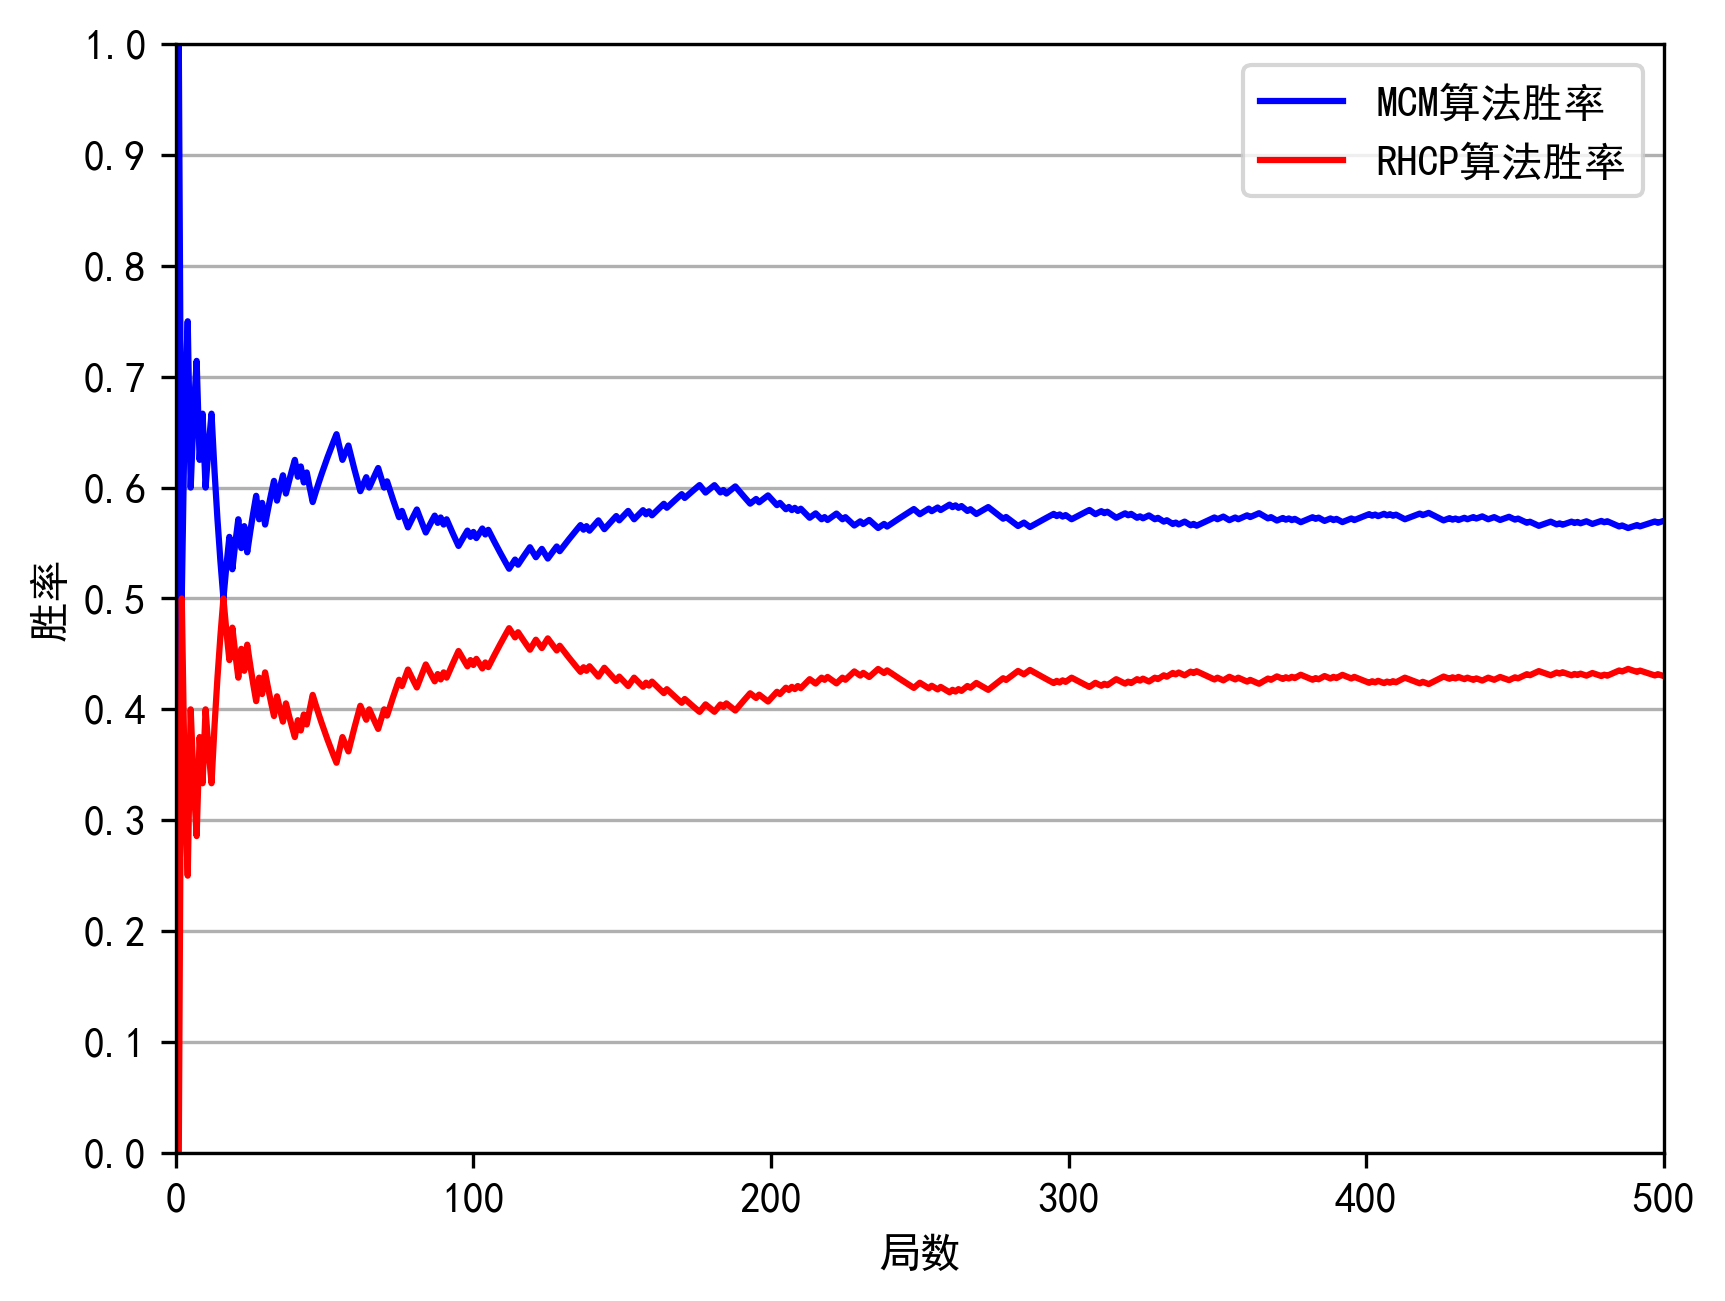
\includegraphics[scale=0.6]{figures/RHCPvMC}
		\end{figure}
	\end{frame}
	
	\begin{frame}
		\frametitle{~~实验结果-----与CQL算法比较}
		\begin{block}{CQL算法介绍}
			~~~~该算法由上海交通大学 You Y 等人提出。You Y 等人针对“斗地主” 博弈中, 每次出牌时存在较多可能组合牌型的情况,提出一种处理组合动作的新方法组合Q学习(CQL)。 
		\end{block}
		\text{地主 MCM 对农民 CQL 的胜率变化图:}\vspace{-0.1cm}
		\begin{figure}
			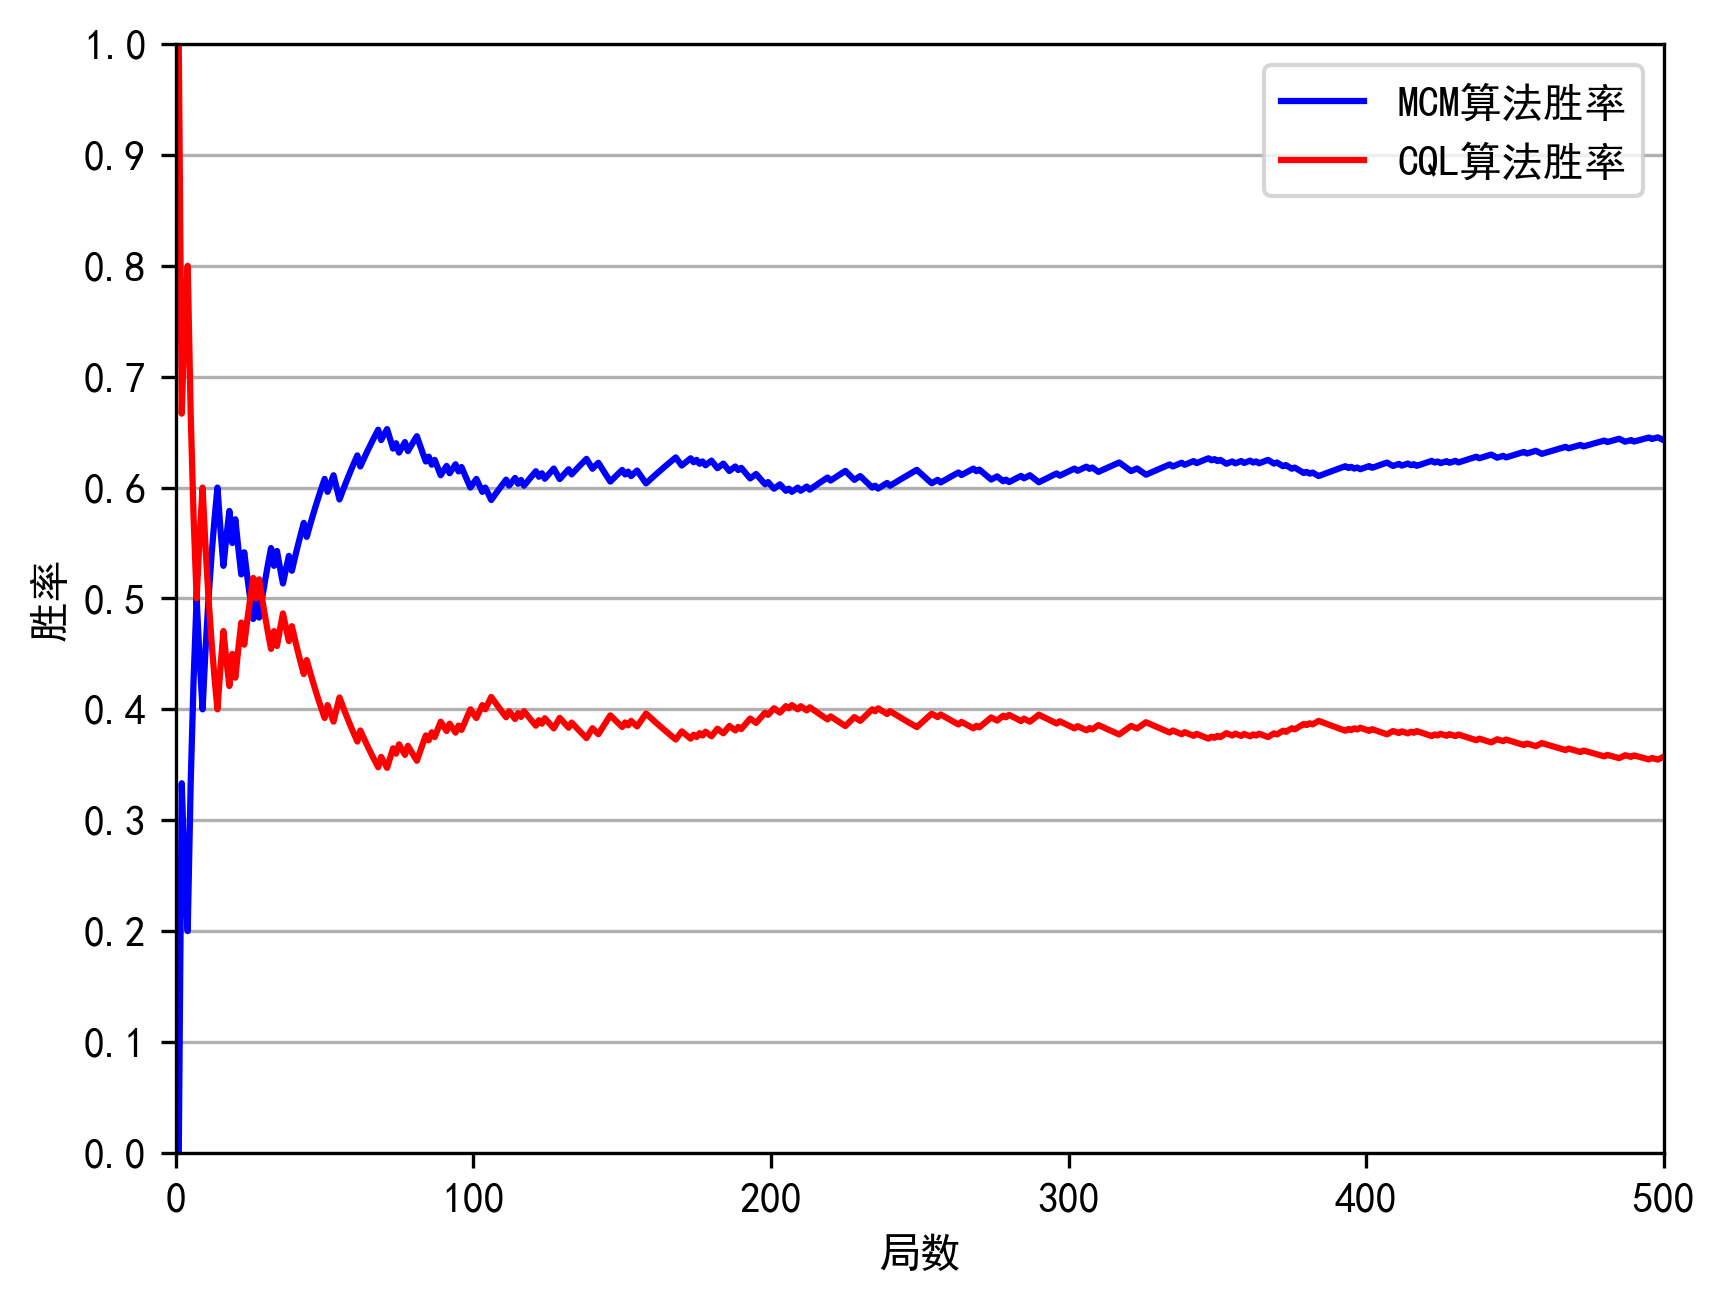
\includegraphics[scale=0.45]{figures/MvC}
		\end{figure}
	\end{frame}
	
	\begin{frame}
		\frametitle{~~实验结果-----与CQL算法比较}
		\text{农民MCM 对地主CQL 的胜率变化图:}\vspace{-0.1cm}
		\begin{figure}
			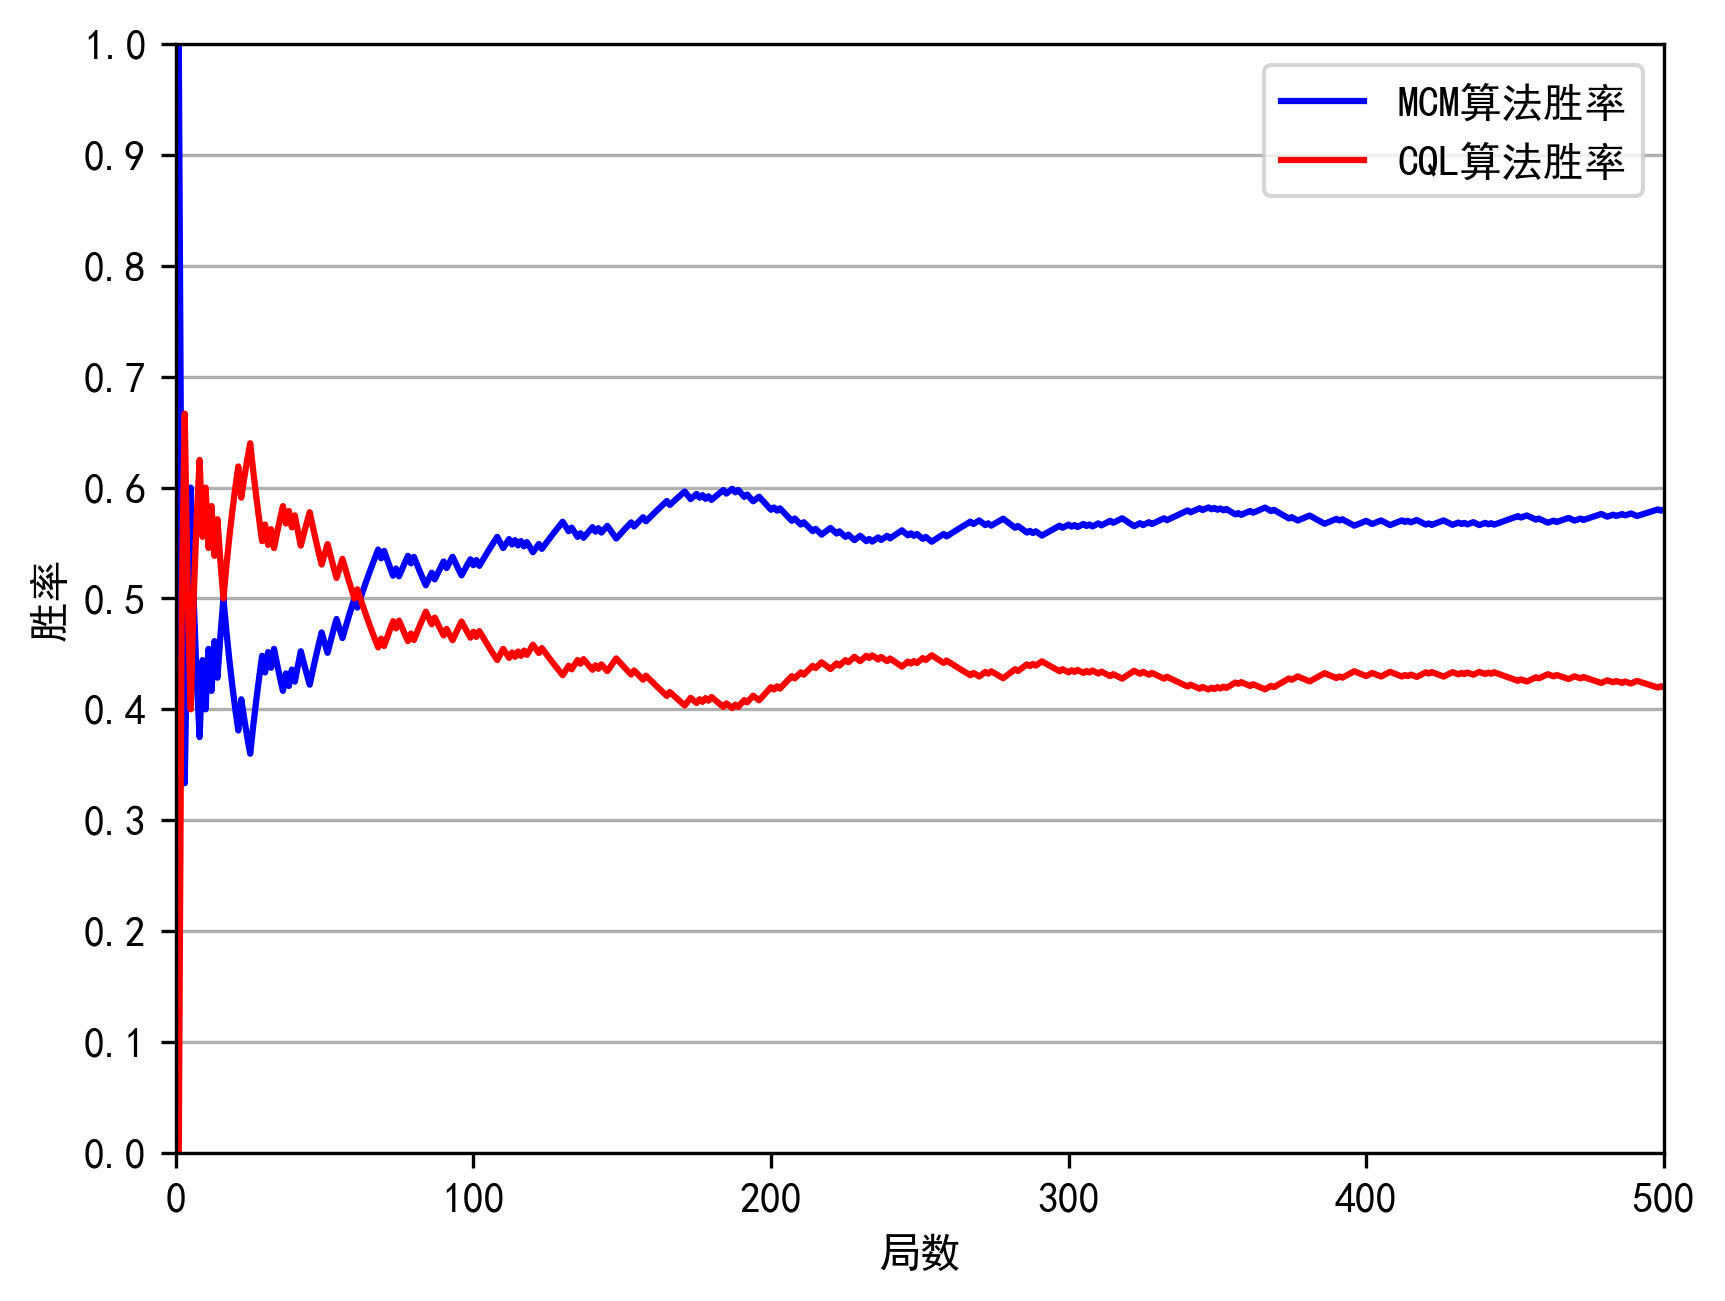
\includegraphics[scale=0.6]{figures/CvM}
		\end{figure}
	\end{frame}
	
	\begin{frame}
		\frametitle{~~实验结果-----CQL、RHCP、MCM相互比较}
		\text{CQL、RHCP以及MCM算法相互比较:}
		\begin{center}
			\begin{tabular}{|c|c|c|c|c|c|}
				\hline 
				\multicolumn{2}{|c|}{地主} & \multicolumn{2}{|c|}{农民一} &  \multicolumn{2}{|c|}{农民二}  \\ 
				\hline 
				决策算法 & 胜率 & 决策算法 & 胜率 & 决策算法 & 胜率 \\ 
				\hline 
				CQL & 44.4\% & RHCP & 21.6\% & MCM & 34\% \\ 
				\hline 
				CQL & 44.8\% & MCM & 21.6\% & RHCP & 33.6\% \\ 
				\hline 
				RHCP & 52.6\% & CQL & 6.4\% & MCM & 41\% \\ 
				\hline 
				RHCP & 46.4\% & MCM & 28\% & CQL & 25.6\% \\ 
				\hline 
				MCM & 63\% & CQL & 6\% & RHCP & 31\% \\ 
				\hline 
				MCM & 59.2\% & RHCP & 26.6\% & CQL & 14.2\% \\ 
				\hline 
				MCM & 56\% & MCM & 22.4\% & MCM & 21.6\% \\ 
				\hline 
			\end{tabular} 
		\end{center}
	\end{frame}
	
	\begin{frame}
		\frametitle{~~实验结果-----CQL、RHCP、MCM相互比较}
		\text{CQL、RHCP以及MCM算法相互比较:}
		\begin{center}
			\begin{tabular}{|c|c|c|c|c|c|}
				\hline 
				\multicolumn{2}{|c|}{地主} & \multicolumn{2}{|c|}{农民一} &  \multicolumn{2}{|c|}{农民二}  \\ 
				\hline 
				决策算法 & 胜率 & 决策算法 & 胜率 & 决策算法 & 胜率 \\ 
				\hline 
				CQL & 44.4\% & RHCP & 21.6\% & MCM & 34\% \\ 
				\hline 
				CQL & 44.8\% & MCM & 21.6\% & RHCP & 33.6\% \\ 
				\hline 
				RHCP & 52.6\% & CQL & 6.4\% & MCM & \multicolumn{1}{>{\columncolor{mycyan}}l}{{\large 41\%}} \\ 
				\hline 
				RHCP & 46.4\% & MCM & \multicolumn{1}{>{\columncolor{mycyan}}l}{{\large 28\%}} & CQL & 25.6\% \\ 
				\hline 
				MCM & \multicolumn{1}{>{\columncolor{mycyan}}l}{{\large 63\%}} & CQL & 6\% & RHCP & 31\% \\ 
				\hline 
				MCM & 59.2\% & RHCP & 26.6\% & CQL & 14.2\% \\ 
				\hline 
				MCM & 56\% & MCM & 22.4\% & MCM & 21.6\% \\ 
				\hline 
			\end{tabular} 
		\end{center}
	\end{frame}
	
	\begin{frame}{~~实验结果-----CQL、RHCP、MCM相互比较}{~~~~(相同牌局)}
		\text{CQL、RHCP以及MCM算法相互比较:}
		\begin{center}
			\begin{tabular}{|c|c|c|c|c|c|}
				\hline 
				\multicolumn{2}{|c|}{地主} & \multicolumn{2}{|c|}{农民一} &  \multicolumn{2}{|c|}{农民二}  \\ 
				\hline 
				决策算法 & 胜率 & 决策算法 & 胜率 & 决策算法 & 胜率 \\ 
				\hline 
				CQL & 42\% & RHCP & 19\% & MCM & \multicolumn{1}{>{\columncolor{mycyan}}l}{{\large 40\%}} \\ 
				\hline 
				CQL & 47\% & MCM & 19\% & RHCP & 34\% \\ 
				\hline 
				RHCP & 57\% & CQL & 10\% & MCM & 32\% \\ 
				\hline 
				RHCP & 52\% & MCM & \multicolumn{1}{>{\columncolor{mycyan}}l}{{\large 31\%}} & CQL & 17\% \\ 
				\hline 
				MCM & 66\% & CQL & 8\% & RHCP & 36\% \\ 
				\hline 
				MCM & \multicolumn{1}{>{\columncolor{mycyan}}l}{{\large 67\%}} & RHCP & 20\% & CQL & 13\% \\ 
				\hline 
			\end{tabular} 
		\end{center}
		\begin{itemize}
			\item \textbf{{\large 上述实验结果详见:}}\\
			https://github.com/StarrySky3/experimental-result-/tree/master/experimental-result
		\end{itemize}
	\end{frame}
	
	\section{总结与展望}
	\subsection*{总结}
	\begin{frame}
		\frametitle{~~总结}
		\text{{\Large 总结:}} 
		\begin{spacing}{1.5}
			\begin{itemize}
				\item 论文提出MCTSHS算法对“斗地主”进行研究。实验表明该算法针对“斗地主”博弈能做出不错的决策。
				\item 针对基于MCTSHS算法的思考时间过长且已搜索策略未能充分利用的缺点,论文提出MCM算法。实验表明,MCM算法相较于其它智能决策算法具有一定优势。
			\end{itemize}
		\end{spacing}
	\end{frame}
	
	\subsection*{展望}
	\begin{frame}
		\frametitle{~~展望}
		\text{\Large 展望:} 
		\begin{spacing}{1.5}
			\begin{itemize}
				\item 后续研究对玩家手牌信息进行预测处理。
				\item 在后续的工作中,可以对玩家进行对手建模。通过预测玩家手牌以实现对手当前状态下的可能决策,从而找到最佳的应对之策以取得游戏胜利。
			\end{itemize}
		\end{spacing}
	\end{frame}
	
	\begin{frame}
		\frametitle{~~参与项目及成果}
		\text{\Large 作者在攻读硕士学位期间参与项目及成果} 
		\begin{spacing}{1.5}
			\begin{itemize}
				\item 发表了一篇中文核心
				\item 申请了一项国家发明专利(在审)
				\item 参加国家自然科学基金1项
			\end{itemize}
		\end{spacing}
	\end{frame}
	
	\begin{frame}
		\centering
		\zihao{2} 敬请各位老师批评指正\\
		\zihao{1} 谢谢!
	\end{frame}
\end{document}